% !TEX TS-program = pdflatex


\documentclass{lncs/llncs}

\usepackage[T1]{fontenc}
\usepackage{geometry}                % See geometry.pdf to learn the layout options. There are lots.
\geometry{a4paper}                   % ... or a4paper or a5paper or ...
%\geometry{landscape}                % Activate for for rotated page geometry
%\usepackage[parfill]{parskip}    % Activate to begin paragraphs with an empty line rather than an indent
\usepackage{graphicx}

%\usepackage{amsfonts}
%\usepackage{fancyhdr}
%\usepackage{cite}
%\usepackage{ifthen}
%\usepackage{amssymb}
%\usepackage{fancyhdr}
%\usepackage{pifont}
\usepackage{stmaryrd}
\usepackage{mathtools,mathpartir}
\usepackage{proof}
%\usepackage{setspace}
%\usepackage{indentfirst}
\usepackage{amsmath,amssymb,amscd,mathrsfs}
% \usepackage{array,booktabs,arydshln,xcolor}
\usepackage{array,booktabs,xcolor}
\DeclareGraphicsRule{.tif}{png}{.png}{`convert #1 `dirname #1`/`basename #1 .tif`.png}
\usepackage{epsfig,color,subfigure,enumitem}
\newcommand{\TODO}[1]{\textcolor{red}{\textbf{[TODO:#1]}}}
\newcommand{\NOTE}[1]{\textcolor{blue}{\textbf{[NOTE:#1]}}}
\newcommand{\ERIC}[1]{\textcolor{blue}{#1}}
\newcommand{\OTvar}{\texttt}
\newcommand{\OTland}{\;\land\ }
\definecolor{airforceblue}{rgb}{0.26, 0.44, 0.56}
\newcommand{\QIN}[1]{\textcolor{airforceblue}{#1}}
\newcommand{\coloncolon}{{:\hspace{-.2ex}:}}
\makeatletter
\newcommand{\raisemath}[1]{\mathpalette{\raisem@th{#1}}}
\newcommand{\raisem@th}[3]{\raisebox{#1}{$#2#3$}}
\makeatother

\usepackage{macrospNets}

\def\AlgT{\mathcal{T}}
\def\AlgE{\mathcal{E}}
\def\AlgA{\mathcal{A}}
\def\AlgAS{\mathcal{A}_S}
\def\AlgB{\mathcal{B}}
\def\AlgI{\mathcal{I}}

\newcommand{\Pred}{\symb{Pred}}
\newcommand{\MkPred}{\symb{MkPred}}
\newcommand{\Post}{\symb{Post}}
%\usepackage[math]{cellspace}
%\setlength\cellspacetoplimit{ 37pt}
%\setlength\cellspacebottomlimit{18pt}

\pagestyle{plain}

% addition to the mathpartir package for red dotted rules,
% that we use for open-transitions

\makeatletter
\def \dotover {\textcolor{red}{\leavevmode\cleaders\hb@xt@ .22em{\hss $\cdot$\hss}\hfill\kern\z@}}
\def \reddottedrule #1#2{\hbox {\advance \hsize by -0.5em
%\sbox0{$\genfrac{}{}{0pt}{0}{#1}{#2}$} \phantom{\copy0} %
 {\ooalign{\vphantom{$\genfrac{}{}{0pt}{0}{#1}{#2}$}\cr\dotover\cr$\genfrac{}{}{0pt}{0}{#1}{#2}$\cr}}}}

 \def \dottedrule #1#2 {
  {\sbox0{$\genfrac{}{}{0pt}{0}{#1}{#2}$}%
    \vphantom{\copy0}%
    \ooalign{%
      \hidewidth
      $\vcenter{\moveright\nulldelimiterspace
        \hbox to\wd0{%
         \xleaders\hbox{\kern.5pt\vrule height 0.4pt width 1.5pt\kern.5pt}\hfill
          \kern-1.5pt
        }%
      }$
      \hidewidth\cr
    \box0\cr}}
}

\let \defaultfraction \mpr@@fraction
\makeatother

%\newtheorem{theorem}{Theorem}[section]
\newtheorem{prop}[theorem]{Proposition}
%\newtheorem{corollary}[theorem]{Corollary}
%\newtheorem{lemma}[theorem]{Lemma}
\newtheorem{alg}[theorem]{Algorithm}
%\newtheorem{remark}[theorem]{Remark}
%\newtheorem{definition}[theorem]{Definition}
%\newtheorem{example}[theorem]{Example}
%\newtheorem{problem}[theorem]{Problem}
%\newtheorem{proof}[theorem]{Proof}

% Macros for the SOS rules and proof trees:
%\newcommand\openrule[2]{\redinfer{#1}{#2}}
\newcommand\openrule[2]{\inferrule*[myfraction=\reddottedrule,center]{#1}{#2}}
%\newcommand\openrule[2]{\inferrule*{#1}{#2}}
%\newcommand\ostate[1]{\triangleleft{\;#1\;}\triangleright}
\newcommand\ostate[1]{\triangleleft{#1}\triangleright}
\newcommand{\sm}[1]{\mbox{\boldmath\small #1}}
\usepackage{algorithm} 
%\usepackage{algorithmicx} 
\usepackage{algpseudocode}  
\renewcommand{\algorithmicrequire}{\textbf{Input:}} 
\renewcommand{\algorithmicensure}{\textbf{Output:}}
\algnewcommand{\IfThen}[2]{\State \algorithmicif\ #1\ \algorithmicthen\ #2}% \IfThenElse{<if>}{<then>}
\algnewcommand{\IfThenElse}[3]{\State \algorithmicif\ #1\ \algorithmicthen\ #2\ \algorithmicelse\ #3}% \IfThenElse{<if>}{<then>}{<else>}
%\DeclareMathOperator{\card}{card}
%\DeclareMathOperator{\Flat}{Flat}
\renewcommand{\P}{\mathcal P}
\usepackage{listings}
\lstset{basicstyle=\small}
%\usepackage{algorithm} 
%\usepackage{algpseudocode} 






\title{Using SMT engine to generate Symbolic Automata\thanks{This work was partially 
funded by the Associated Team FM4CPS
  between INRIA and ECNU, Shanghai}}
\author{ Xudong Qin\inst{2,3}  \ \ \  Eric Madelaine\inst{1,2}
  \ \ \  Min Zhang\inst{3}} 
\institute{Univ. of Nice Sophia Antipolis, CNRS, UMR 7271, 06900 Sophia Antipolis, France
	\and INRIA Sophia Antipolis M\'edit\'erann\'ee, BP 93, 06902 Sophia Antipolis, France
\and Shanghai Key Laboratory of Trustworthy Computing, ECNU, China}
\date{}                                           % Activate to display a given date or no date

                          % Activate to display a given date or no date


\begin{document}

\maketitle

%\section{}
%\subsection{}


\begin{abstract}
  \TODO{not good for a FM, (to be rewriten by Eric)}

  Open pNets are used to model the behavior of open
  synchronous or asynchronous systems expressed in various calculi
  or languages. They are endowed with a symbolic operational semantics
  in terms of so-called ``Open Automata''. We implement an algorithm
  computing this semantics, and building predicates expressing the
  synchronization conditions allowing some combination of events in
  the pNet system. Checking such predicates requires symbolic
  reasoning over first order logics, and specific functions of each
  action algebra. To reduce the complexity of the generated open
  automata, we use the Z3 SMT engine to check satisfiability of the
  predicates, and minimize the number of significant symbolic
  transitions.
  

\end{abstract}


\section{Introduction}

In the nineties, several 
works extended the basic behavioral models based on labelled
transition systems to address value-passing or parameterized systems, using
various symbolic encodings of the
transitions~\cite{deSimone85,Larsen87,HennessyLin:TCS95,Linconcur96}. 
In \cite{Linconcur96}, H.M. Lin addressed value-passing calculi, for which he
developed a symbolic behavioral semantics, and proved algebraic properties.
Separately J. Rathke~\cite{HennessyRathke:TCS98} defined another
symbolic semantics for 
a parameterized broadcast calculus, together with strong and weak bisimulation
equivalences, and developed a symbolic model-checker based on a tableau
method for these processes. Thirty years later, no
practical verification approach and no verification platform are
using this kind of approaches to provide proof methods for
value-passing processes or open process expressions. 

Parameterized Networks of Synchronized Automata (pNets) were proposed
to give a behavioral specification formalism for distributed
systems, synchronous, asynchronous, or heterogeneous. It is used in
VerCors, a platform for designing and 
verifying distributed systems, as the intermediate language for various
high-level languages. The high-level languages in VerCors formalize
each component of the 
distributed system and gives out the composition of these
components.
pNets provides the core low-level semantic formalism for VerCors, and
is made of a hierarchical composition of (value-passing) automata,
called parameterized labelled transition systems (pLTS), where each
hierarchical level defines the possible synchronization of the lower levels.
Traditionally, pNets have been used to formalize fully
defined systems or softwares. But we want also to define and reason
about incompletely defined systems, like program skeletons, operators,
or open expressions of process calculi.
The open pNet is proposed to solve the
problem of the undefined components contained in the systems using
"holes" as the process parameter dealing with these components. The
hole acts as the placeholder for the uncertain component with a set of
possible behaviors the component might conduct, presenting the "open"
property.  
The pNet model was developed in a series of
papers~\cite{HMZ:PDP15,henrio:Forte2016} in which many examples have been
introduced showing its ability to encode the operators from some
other algebras or  program skeletons.
The operational semantic of an (open) pNet is defined as an
Open Automaton in which Open Transitions contain logical predicates
expressing the relations between the behavior of the holes, and the
global behavior of the system. In the previous publication,
only a sketch of a procedure allowing to compute this semantics was
presented, together with a proof of finiteness of the open automaton, under
reasonable hypotheses on the pNet structure.

Implementing this semantics raised several challenges, in order:
\begin{itemize}
  \item to get a tool that could be applied to pNets representing
    various languages, in particular various actions algebras,
    with their specific decision theories,
  \item to separate clearly on one hand the algorithmic part, as an
      algorithm generating the transitions of the open automaton from
      combination of all possible (symbolic) behaviors; on the other hand
      the symbolic reasonning part, specificaly here using an SMT
      engine to check the
      satisfiability of the predicates generated by our algorithm,
  \item to build a prototype and validate the approach on our basic
    case-studies, and understand the efficiency of the interaction
    with the SMT solver.
\end{itemize}

In the long goal, we want to be able to check the equivalence between
open systems encoded as pNets. The equivalence between pNets is
"FH-bisimulation" taking the 
predicate of the open transitions into account each time matching such
open transitions. We foresee that the interplay with the SMT solver
that we use here for satisfiability of open transitions will be
similar with what we need to prove (symbolic) equivalence between open
transitions. 

%% This paper presents our open automaton computing algorithm and its
%% implementation using the pNet API from the VerCors platform.
%% Comparing
%% the result of the algorithm with 
%% the manual result on our running examples shows that the algorithm
%% works properly in computing the pNet semantics.
%% The
%% algorithm contains the method computing the open transitions composing
%% the transitions from the subnets according to several defined rules
%% the open transitions need to satisfy. These results are not the final
%% results in fact, because they contain some unsatisfiable results we need
%% to eliminate. To eliminate those unsatisfiability, we interact with an
%% automatic theorem prover for satisfiability checking.

\paragraph{Contribution}
In the article we show how:
\begin{itemize}
\item We define the open automaton generation algorithm, and we
  implemented a full working prototype, within the 
  VerCors platform. In the process, we improved the
  semantics rules from~\cite{henrio:Forte2016}, and add features in
  the algorithm to deal the full 
  model, including management of variables and assignments.
%  \item We extended the meta-model of action expressions, and the
%    associated API, in the VerCors platform, to be able to manage
%    parameterisation over the action algebra operators.
\item We implement the interaction between our algorithm and the Z3
    SMT solver, for checking satisfiability of the transitions
    generated by the algorithm.
  \item \ERIC{We show the interest of this approach on an
    industrial-inspired use-case, namely one architectural pattern
    extracted from the BIP specification of a nano satellite on-bord
    software.} 
\end{itemize}





\paragraph{Related works}

%% \TODO{say that apart from the old work by J. Rathke, we know no other
%%   research addressing our goals, and especially no attempts to develop
%%   an algorithmic treatment of such symbolic systems by interacting
%%   with automatic theorem provers}.

%% \TODO{Then you can list the ATP/ITP you have mentioned Coq, Isabelle,
%%   B-tools, or others like CVC4, as possible alternative to Z3}


There is not much research work towards trying to develop symbolic bisimulation approaches
for the value-passing process algebra and languages, as our long-term goals,
especially no algorithm treatment of the symbolic systems developed by
interacting with automatic theorem provers. The closest work is the
one already mentioned from J. Rathke~\cite{HennessyRathke:TCS98},
who developed the symbolic bisimulation for a
calculus of broadcasting system (CBS). CBS is similar with classic
process calculi such as CCS and CSP, but communicating by broadcasting
values, one-to-many communication instead of one-to-one communication
and transmitting values without blocking. That makes the definition of
the symbolic semantic and bisimulation equivalence different from the
classic works.


For other applications, e.g. for the analyses of 
programming languages, there exist dedicated platforms making use of
external automatic theorem 
provers (ATP), or even some automatic tactics from interactive theorem
provers (ITP), to perform symbolic reasoning, and for example to
discharge some subgoals in the proofs.
Tools like Rodin~\cite{deharbe2013,deharbe2014,abrial2007} have
already integrated several provers, like Z3, as modules for proving
the proof obligations generated from the model inputed by user. 
The prover we used, which also happens to be Z3, is developed by Microsoft Research
based on the satisfiability modulo 
theories (SMT), mainly applied in extended static checking, test case
generation, and predicate abstraction.
In a similar way, there are several ATPs/ITPs we could consider to use for
the result pruning and bisimulation checking in our algorithm, as an
alternative to Z3, such as CVC4~\cite{barrett:CAV2011},
Coq~\cite{armand:CPP2011},
%Coq~\cite{armand:CPP2011,besson:CPP2011},
Isabelle~\cite{blanchette:FroCoS2011} or others. 


\paragraph{Structure.}
In section
\ref{section:pnets} we give a description and a formal definition of
the pNet model, as found in previous publications. Then in
\ref{section:examples} we present a simple example that will
illustrate the rest of the paper.
Section \ref{section:op-semantics} recalls the operational semantics
of pNet, including its structural rules.
%, and a sketch of the algorithm
%to compute such semantics, but also explains the enhancement we have
%done to these definitions
Section \ref{section:implementation} explains in details our
implementation within the Vercors platform, and shows the full result of
the semantic computation on the running example.
Finally we conclude and discuss perspectives in section
\ref{section:conclusion}. 




\section{Background: pNets definition}
\label{section:pnets}

\TODO{To be reduced, moving more material to the appendix}
  
This section introduces pNets and the notations we will use in
this paper. Then it gives the formal definition of pNet structures,
together with an operational semantics for open pNets.

pNets are tree-like structures, where the leaves are either
\emph{parameterized labelled transition systems (pLTSs)}, expressing the
behavior of basic processes, or \emph{holes}, used as placeholders
for unknown processes, of which we only specify their set of possible
actions, named \emph{sort}.
Nodes of the tree (pNet nodes) are synchronizing artifacts, using a
set of \emph{synchronization vectors} that express the possible
synchronization between the parameterized actions of a subset of the
sub-trees.


%\smallskip\noindent
\paragraph*{Notations.}
We extensively use indexed structures
over some countable indexed sets, which are equivalent to mappings over
the countable set. % . The indexes will usually be
% integers, bounded or not. Such an indexed family is
%denoted
%follows:
$a_i^{i\in I}$
%, or equivalently  $(i\mapsto a_i)^{i\in I}$
denotes a family of elements $a_i$ indexed over the
set $I$. % Such a family
% is equivalent to the mapping $(i\mapsto a_i)^{i\in I}$.
% To specify the set over which the structure is indexed,
% indexed structures are always denoted with an exponent of the form $i\in I$
% (arithmetic only appears in the indexes if necessary).
$a_i^{i\in I}$ defines both $I$ the set over which the family is
indexed (called \emph{range}), and $a_i$ the elements of the family.
E.g., $a^{i\in\{3\}}$ is the mapping with a single entry $a$ at index
$3$ ; abbreviated $(3\mapsto a)$ in the following.
When this is not
ambiguous, we shall use notations for sets, and typically write
``indexed set over I'' when formally we should speak of multisets, and
write $x\in a_i^{i\in I}$ to mean $\exists i\in I.\, x=a_i$.  An empty
family is denoted $\emptyset$. We
denote classically $\overline{a}$ a family when the indexing set is
not meaningful.  $\uplus$ is the disjoint union on
indexed sets.


\paragraph*{Term algebra.}
Our models rely on a notion of parameterized actions, that are
symbolic expressions using data types and variables. As our model aims
at encoding the low-level behavior of possibly very different
programming languages, we do not want to impose one specific algebra
for denoting actions, nor any specific communication mechanism. So we
leave unspecified the constructors of the algebra that will allow building
expressions and actions. Moreover, we use a generic {\em action interaction}
mechanism, based on unification between two or more action
expressions. This will be used in the semantics of synchronization
vectors to express various kinds of communication or synchronization mechanisms.

\def\Talg{\mathcal{T}_{\Sigma,\P}}
Formally, we assume the existence of a term algebra $\Talg$,
where $\Sigma$ is the signature of the data and action constructors,
and $\P$ a set of variables. Within $\Talg$, we distinguish a set of
data expressions $\mathcal{E}_\P$, including a set of boolean
expressions $\mathcal{B}_{\P}$ ($\mathcal{B}_{\P}\subseteq\mathcal{E}_\P$).
On top of $\mathcal{E}_\P$ we build the action algebra
$\mathcal{A}_\P$, with $\mathcal{A}_P\subseteq\mathcal{T}_\P,
\mathcal{E}_P\cap\mathcal{A}_P=\emptyset$;
naturally action terms will use data expressions as sub-terms.
The function $\vars(t)$ identifies the set of variables in a term
$t\in\AlgT$.


pNets can encode naturally the notion of input actions as found e.g. in value-passing CCS
\cite{Milner89} or of usual point-to-point message passing calculi, but it also allows
for more general mechanisms, like gate negotiation in Lotos, or broadcast
communications.
\QIN{
\paragraph*{Algebra presentations}
\begin{definition}
  An Algebra Presentation is a pair $\mathcal{P}=<Sorts,Constrs,Ops>$ where:
  \begin{itemize}
  \item $Sorts$ is a set of Sort names
    \footnote{Later we may want to extend this with Sort constructors,
      like Array or Pair, but this is not needed now}
  \item $Constrs$ is a set of constructor operators, with $Con$ the
    constructor name, and arity: $arity(Con)=n \in \mathbb{N}$,
    and with their signature and their associated selectors,
    of the form: '$Con : (sel_1,sort_1), ... , (sel_n,sort_n) -> sort$'.
    For each argument, the pair $(sel_i,sort_i)$ defines an auxiliary
    operator of name $sel_i$ with signature $sel_i : sort -> sort_i$.
    \item $Ops$ is a set of other (auxiliary) operators, with their
      arity and signature, of the form: $Op : sort_1, ...  sort_n ->
      sort$
      \item $Constrs(sortname), Sels(sortname)$, respectively define the set of
        constructors and selectors of sort $sortname$
  \end{itemize}
  All sorts and operator names must be distinct.\\
  Amongst Constructors, those of arity 0 are called constants, and we
  define $Consts(\mathcal{P}) = \{Con \in Constrs. arity(Con)=0\}$.
\end{definition}
}

\subsection{The (open) pNets Core Model}
\label{section:pNets}


A pLTS is a labelled transition system with variables; variables can be
manipulated, defined, or accessed inside states, actions, guards, and
assignments. 

%Without loss of generality and to simplify the formalization, we suppose 
%here that variables are local to 
%state: each state has its set of variables disjoint from the others. Transmitting 
%variable values from one state to the other can be done by explicit assignment. 

Each state has its set of variables called $State\ variables$, 
which can only be modified by the assignment in the transitions targeting its owner state. 
A global state variable of a pLTS is a variable $x$ satisfying $\forall s\!\in\! S .\, x\!\in\! \vars(s)$.

%Similarly, to simplify the management of variables and without loss of expressivity, we 
%suppose that transitions looping to the same state does not do assignments.
Note that we make no assumption on finiteness of the set of states nor
on finite branching of the transition relation.

We first define the set of actions a pLTS can use, let $a$
range over action labels, $\symb{op}$ are operators, and $x_i$ range over
variable names. Action terms are:
\[
\begin{array}[l]{rcl@{\quad}p{5.5cm}}
  \alpha\in\AlgA&::=&a(p_1,\ldots,p_n)&\text{action terms}\\
  p_i&::=& ~\symb{Expr}&\text{parameters}\\
  \symb{Expr}&::=& \symb{Value}~|~x~|~\symb{op}(\symb{Expr}_1,..,\symb{Expr}_n)&\text{Expressions}
\end{array}
\]
%\[
%\begin{array}[l]{rcl@{\quad}p{5.5cm}}
%  \alpha\in\AlgA&::=&a(p_1,\ldots,p_n)&\text{action terms}\\
%  p_i&::=& ?x~|~\symb{Expr}&\text{parameters (input variable or expression)}\\
%  \symb{Expr}&::=& \symb{Value}~|~x~|~\symb{op}(\symb{Expr}_1,..,\symb{Expr}_n)&\text{Expressions}
%\end{array}
%\]

%% \QIN{
%% [The input variables in an action term are those marked with a
%% $\symb{?}$.
%% We additionally suppose that each input variable does not
%% appear somewhere else in the same action term:
%% $p_i=?x\Rightarrow\forall j\neq i.\, x\notin \vars(p_j)$]}

\begin{definition}[pLTS]
\label{pLTS}
A pLTS is a tuple
$pLTS\triangleq\mylangle S,s_0, \to\myrangle$ where:
\begin{itemize}
\item[$\bullet$]
$S$ is a set of states.
\item[$\bullet$]
$s_0 \in S$ is the initial state.
\item[$\bullet$] $\to \subseteq S \times L \times S$ is the transition relation and 
$L$ is the set of labels of the form
$\langle \alpha,~e_b,~(x_j\!:= {e}_j)^{j\in J}\rangle$,
where $\alpha \in\AlgA$ is a parameterized action, $e_b \in
\AlgB$ is a guard, and the variables $x_j\in P$
are assigned the expressions $e_j\in \AlgE$.
If 
$s \xrightarrow{\langle \alpha,~e_b,~(x_j\!:= {e}_j)^{j\in
		J}\rangle} s'\in \to $ then 
		$\vars(\alpha)\!\subseteq\! \vars(s)$, 
		$\vars(e_b)\!\subseteq\! \vars(s')$, and
		$\forall j\!\in\! J .\,\vars(e_j)\!\subseteq\! \vars(s)\land 
x_j\!\in\!\vars(s')$.
\item[$\bullet$]
The $x_j$ here are $state\ variables$ of state $s'$. 


\end{itemize}
\end{definition}

Now we define
pNet nodes, as constructors for hierarchical behavioral structures.
A pNet node has a set of sub-pNets that can be either pNets or pLTSs, and a
set of Holes, playing the role of process parameters.

A composite pNet consists of a set of sub-pNets exposing
a set of actions, each of them triggering internal actions in each of
the sub-pNets. The synchronization between global actions and
internal actions is given by  \emph{synchronization vectors}: a
synchronization vector synchronizes one or several internal actions, and
exposes a single resulting global action.


\begin{definition}[pNets]\label{def-pnets}
A pNet is a hierarchical structure which leaves are pLTSs and holes:\\
$\pNet\triangleq pLTS~|~\mylangle \pNet_i^{i\in I}, S_j^{j\in J}, \symb{SV}_k^{k\in K}\myrangle$
where
\begin{itemize}
\item[$\bullet$] $I \in \I$ is the set over which sub-pNets are indexed.
\item[$\bullet$] $\pNet_i^{i\in I}$ is the family of sub-pNets.

\item[$\bullet$] $J\in\I_\P$ is the set over which holes are indexed.
$I$ and $J$ are \emph{disjoint}: $I\cap J=\emptyset$,  $I\cup J\neq\emptyset$

\item[$\bullet$] $S_j \subseteq \AlgA$ is a set of action terms,
  denoting the $\Sort$\footnote{The formal definition of $Sorts$ (set of actions of a Hole
  or pNet), $Leaves$ and $Holes$ (all pLTSs (resp holes) in a pNet
  hierarchical system. These can be found in \cite{henrio:Forte2016}.}
  of hole $j$. 

\item[$\bullet$] $\symb{SV}_k^{k\in K}$ is a set of
  synchronization vectors ($K\in\I_\P$). $\forall k\!\in\! K,
  \symb{SV}_k\!=\!\alpha_{l}^{l\in I_k \uplus J_k}\to\alpha'_k$ where
  $\alpha'_k\in \mathcal{A}_\P$, $I_k\subseteq I$, $J_k\subseteq J$,
  $\forall i\!\in\! I_k.\,\alpha_{i}\!\in\!\Sort(\pNet_i)$,
  $\forall j\!\in\!
  J_k.\,\alpha_{j}\!\in\!S_j$, and $\vars(\alpha'_k)\subseteq \bigcup_{l\in I_k\uplus 
  J_k}{\vars({\alpha_l})}$. The global action of a vector $\symb{SV}_k$ is
$\Label(\symb{SV}_k) = \alpha'_k$.


\end{itemize}
\end{definition}


%The preceding definition relies on the auxiliary functions below:

%\begin{definition}[Sorts, Holes, Leaves of pNets]
%  \begin{itemize}
%  \item The sort of a pNet is its signature, i.e. the set of actions it can
%perform. In the definition of sorts, we do not need to distinguish
%input variables (that specify the dataflow within LTSs), so for
%computing LTS sorts, we use a substitution operator\footnote{$\subst{y_k\gets x_k}^{k\in K}$ is the parallel substitution 
%operation.} to remove the
%\emph{input marker} of variables. Formally:
%\[
%\begin{array}{l}
%\Sort(\mylangle S,s_0, \to\myrangle) = \{\alpha\subst{x \gets ?x| 
%x\in\symb{iv}(\alpha)}|s \xrightarrow{\langle \alpha,~e_b,~(x_j\!:= {e}_j)^{j\in
%		J}\rangle} s'\in \to \} \\ \Sort(\mylangle
%\set{\pNet}, \set{\symb{S}}, \set{\symb{SV}}\myrangle) =\{\alpha'_k |\, \alpha_j^{j\in J_k}\to\alpha'_k\in\set{\symb{SV}}\}
%\end{array}
%\]
%
%\item
%The set of holes of a pNet is defined inductively; the sets of holes
%in a pNet node and its subnets are all disjoint:
%  \[\begin{array}{l}
%\Holes(\mylangle S,s_0, \to\myrangle) \!=\! \emptyset \\
%\Holes(\mylangle \pNet_i^{i\in I}\!,S_j^{j\in J}\!, \overline{\symb{SV}}\myrangle) =J\cup{\displaystyle \bigcup_{i\in I}\Holes(\pNet_i)}\\
%\forall i\in I.\, \Holes(\pNet_i)\cap J=\emptyset\\
%\forall i_1,i_2\in I.\,i_1\neq i_2\Rightarrow  \Holes(\pNet_{i_1})\cap\Holes(\pNet_{i_2})=\emptyset
%\end{array}\]
%\item
%The set of leaves of a pNet is the set of all pLTSs occurring in the structure, defined inductively as:
%\[\begin{array}{l}
%\Leaves(\mylangle S,s_0, \to\myrangle) \!=\! \{ \mylangle S,s_0, \to\myrangle \}\\
%\Leaves(\mylangle \pNet_i^{i\in I}\!,S_j^{j\in J}\!, \overline{\symb{SV}}\myrangle) = {\displaystyle \bigcup_{i\in I}\Leaves(\pNet_i)}
%\end{array}\]
%\end{itemize}
%\end{definition}
%
%A pNet $Q$ is \emph{closed} if it has no hole: $\Holes(Q)=\emptyset$; else it
%is said to be \emph{open}.


%% \begin{figure}[t]
%% \begin{minipage}{6.1cm}

%%   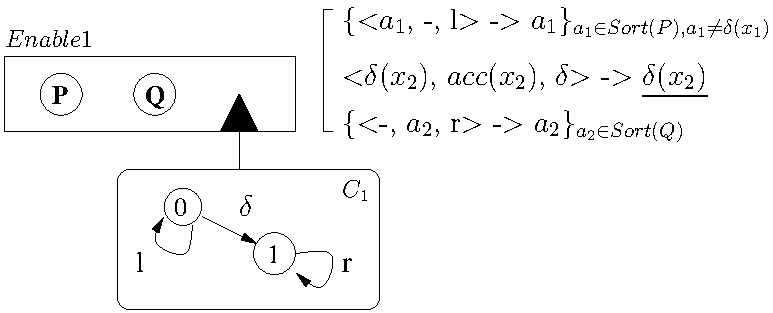
\includegraphics[width=\linewidth]{XFIG/Enable1}
%%   \\[1.3ex]
%%  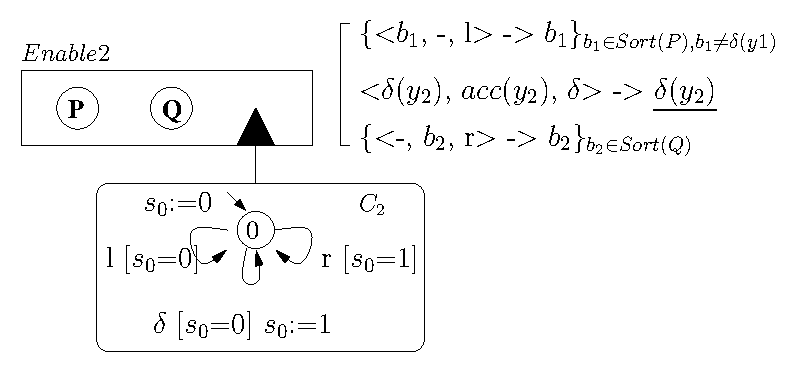
\includegraphics[width=\linewidth]{XFIG/Enable2}
%%   \caption{Two pNet encodings for  Enable }  \label{schema:enable-pnets}
%% \end{minipage}
%%   \hspace{2mm}
%% \begin{minipage}{6cm}
%%   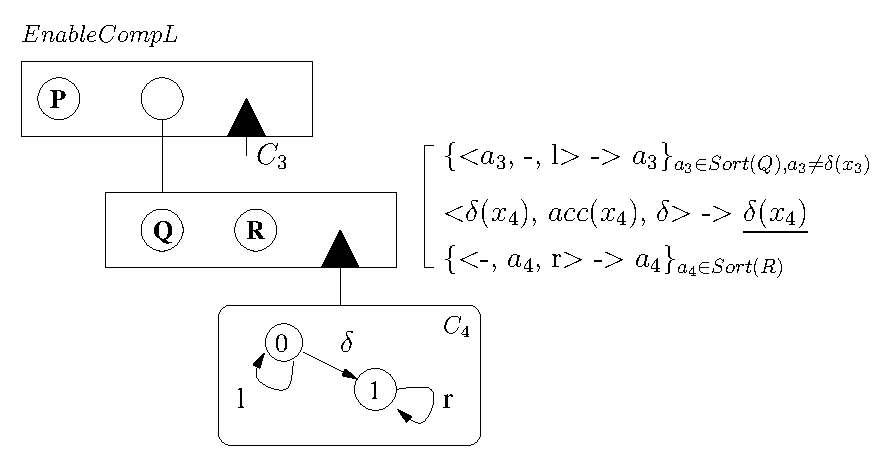
\includegraphics[width=\linewidth]{XFIG/P-QR}
%%   \caption{Composed pNet for ``P>>(Q>>R)''}  \label{schema:enable-composed}
%% \end{minipage}

%% \end{figure}


\section{BIP architectures, and their encodings into pNets}
\label{section:BIParchitectures}

\section{Running example}
\label{section:FailureTimerMax}

Several publications \cite{HMZ:PDP15,henrio:Forte2016} already have introduced
many examples of pNets, encoding
operators of various classical process algebras, or more complex
synchronization structures in distributed or parallel languages.


 \begin{figure}[t]
   \centerline{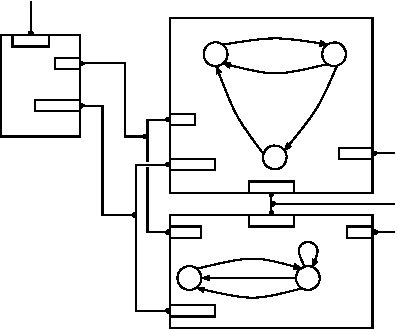
\includegraphics[width=12cm]{XFIG/BIPspec-ArchFailureTimerMax}}
   \caption{FailureTimer Architecture in BIP graphical syntax}  \label{schema:BIParchitecture}
 \end{figure}

\begin{figure}[t]
   \centerline{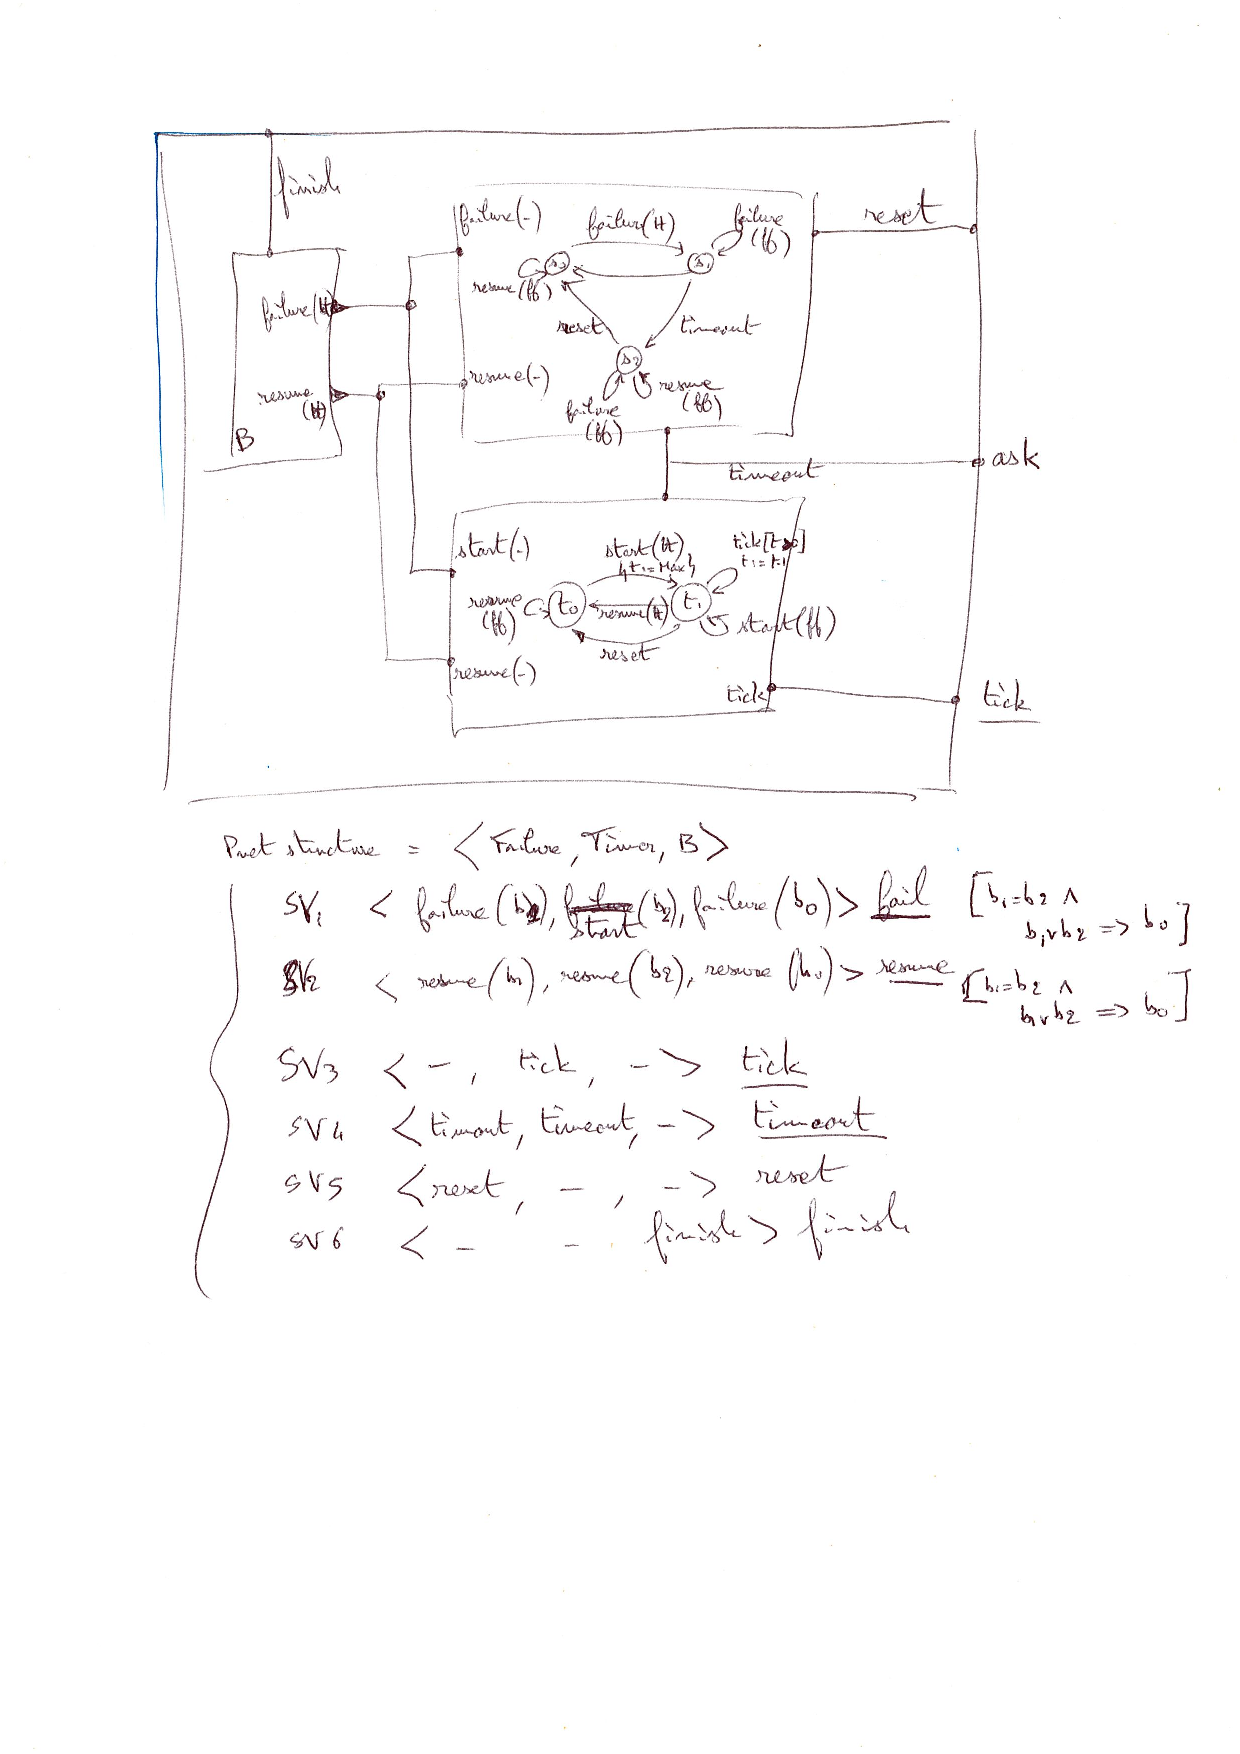
\includegraphics[width=12cm]{XFIG/BIPpnet-ArchFailureTimerMax}}
   \caption{FailureTimer pNet encoding}  \label{schema:BIParchitecture}
 \end{figure}



\section{Operational Semantics for Open pNets}
\label{section:op-semantics}

The semantics of open pNets will be defined  as an open automaton. An open
automaton is an automaton where each transition composes transitions
of several LTSs with the
actions of some holes; the transition occurs if some predicates hold,
and can involve a set of state modifications.

\begin{definition}[Open transitions]
	\label{def:OpenTransitions}
	An \emph{open transition} over a set  $(S_i,s_{0 i}, \rightarrow_i)^{i\in
	I}$ of LTSs, a
	set $J$ of holes with sorts $Sort_j^{j\in J}$, and a set of states $\mathcal{S}$ is a structure of the form:	
	\begin{mathpar}
	\inferrule*[myfraction=\reddottedrule]
	{\{s_i~{\xrightarrow{a_i}}_i ~s_i^{\prime}\}^{i\in I},
		\{\xrightarrow{b_j}_j\}^{j\in J}, \Pred, \Post}
	{s \xrightarrow {v}s'}
	\end{mathpar}
	Where $s, s'\in\mathcal{S}$ and for all
        $i\in I$, $s_i{\xrightarrow{a_i}}_i s_i^{\prime}$ is a transition of the
	LTS $(S_i,s_{0 i}, \rightarrow_i)$, and $\xrightarrow{b_j}_j$
        is a transition of the hole $j$, for any action $b_j$ in the
        sort $Sort_j$. \Pred\ is a predicate
	over the variables of the terms, labels, and states $s_i$,
        $b_j$, $s$, $v$. \Post\ is a set of equations that  
	hold \emph{after the open transition}, represented as a
        substitution $\{x_k\gets e_k\}^{k\in K}$  
	where $x_k$ are variables of $s'$, $s'_i$, and $e_k$ are
        expressions over the other variables of the open transition.
\end{definition}


\begin{definition}[Open automaton]
	\label{def:open-automaton}
	An \emph{open automaton} is a structure\\ $A =
	<LTS_i^{i\in I},J,\mathcal{S},s_0,\mathcal{T}>$ where:
	\begin{itemize}
		\item[$\bullet$]  $I$ and $J$ are  sets of indices,
		\item[$\bullet$]  $LTS_i^{i\in I}$ is a family of LTSs,
		\item[$\bullet$]   $\mathcal{S}$ is a set of states and $s_0$ an initial state
		among $\mathcal{S}$,
		\item[$\bullet$] $\mathcal{T}$ is a set of open transitions and for each
		$t\in \mathcal{T}$ there exist $I'$, $J'$ with $I'\subseteq I$, $J'
		\subseteq J$, such that $t$ is an open transition over $LTS_i^{i\in I'}$, $J'$,
		and  $\mathcal{S}$.
		
	\end{itemize}
\end{definition}
	

%
%Then the semantics of a pNet is characterized by a set of {\em open
%transitions}, where the hypotheses on process parameters are
%replaced by 1) transitions of the pLTSs at the leaves, and 2) formal
%hypotheses on the transitions of the holes. A {\em predicate} is used
%to relate the parameters and names appearing in the actions of the
%leaves and the holes involved in the rules, but also appearing in  the resulting action.

% \TODO{Relate to the algorithm, or even move to section 5}
When building an Open Automaton as the semantics of a pNet, its
\emph{states}, and the shape of the \emph{predicates} in its
transitions have a specific structure:

\paragraph{States of open pNets:}\label{def-states}
  A state of an open pNet is a tuple of the
  states of its leaves (in which we denote tuples
  in structured states as $\triangleleft\ldots\triangleright$).
  For any pNet p, let $\overline{Leaves} = \mylangle S_i,{s_i}_0, \to_i\myrangle^{i \in L}$ be the set of pLTS at its leaves,
  then $States(p) = \{\triangleleft s_i^{i\in L}
  \triangleright| \forall i\in L. s_i \in S_i\}$.
A pLTS being its own single leave:
  $States(\mylangle S,s_0, \to\myrangle) = \{\triangleleft s \triangleright| s \in S\}$.
The initial state is defined as:
$InitState(p) = \triangleleft {{s_i}_0}^{i\in L}  \triangleright$.


%% \begin{example} \emph{State of a pNet}
%%   The states of pNet \texttt{EnableCompL} are:
%%   $\triangleleft 00 \triangleright, \triangleleft 10 \triangleright, \triangleleft 11 \triangleright$
%% \end{example}

\paragraph{Predicates:}
Let
$\mylangle\overline{\pNet},\overline{S},\symb{SV}_k^{k\in K} \myrangle$
be a pNet. Consider a synchronization vector $SV_k$, for $k\in K$. We build a
predicate $\MkPred$ relating
the actions of the involved sub-pNets and the resulting actions. This predicate verifies:
\[\MkPred(SV_k, a_i^{i\in I}, b_j^{j\in J}, v)\Leftrightarrow
\begin{array}{l}
\exists {(a'_i)}^{i\in I},
{(b'_j)}^{j\in J},v'.\, SV_k={(a'_i)}^{i\in I}, {(b'_j)}^{j\in J}\rightarrow v'
\\~~\land
\forall i\in I.\, a_i=a'_i\land \forall j \in J.\, b_j=b'_j \land v=v'
\end{array}\]
%% In any other case (if the action families do not match or if there is no valuation of
%% variables such that the above formula can be ensured) the predicate is undefined.

%% This definition is not constructive but it is easy to build the
%% predicate constructively by brute-force unification of the sub-pNets
%% actions with the corresponding vector actions, possibly followed by a simplification
%% step. 

%\begin{example}\emph{An open-transition.}
%  \label{OT:lotos-composed}
%
%The \texttt{LOTOS} pNet of Fig. \ref{schema:lotos-pnet} has 2
%controllers and 2 holes. We will show its full open Automaton in
%section \ref{section:full-result}. We give one of its transitions here:
%
% \smallskip
% $ ot_2  = \openrule{
%                       \{0 \xrightarrow{\delta}_{C_1} 0, 0 \xrightarrow{acc(x)}_{C_2} 1\}, ~~
%                       \{\xrightarrow{hb_{12}}_P\}, ~~ 
%                        [s_0=0 \!\land\! hb_{12}=\delta(x)], ~~ 
%                       \{s_0 \xleftarrow{} 1\}     
%                      }
%     {\ostate{00} \xrightarrow{\underline{\delta(x)}} \ostate{01}}$
%\end{example}
%
%The open transition $ot_2$ involves the possible actions from the process $P$ and prefix expression $acc(x);Q$. The hole behavior, represented by variable $hb_{12}$ must be equal to the exit action $\delta(x)$, and the accept event $acc(x)$ will capture the same value $x$.
%
%The transition in the conclusion of this rule starts in
%state $\ostate{00}$, where both $C_1$ and $C_2$ are in their initial
%states. It ends in a different structured state, because in $ot_2$
%both pLTS conduct transitions, showing that the control has gone from
%processes $P$ to $(acc(x);Q$, consuming actions $\delta(x)$ and
%$acc(x)$. Controller $C_1$ has only one state, but its state variable
%$s_0$ has changed to 1.


\paragraph{Structural Semantic Rules:}
Now we build the semantics of an open pNet as an open automaton where
LTSs are the pLTSs at 
the pNet leaves, and the states are structured as in
the previous section. 
%given by Definition~\ref{def-states}.
To build an open transition one first
 projects the global state into states of the leaves, then applies
pLTS transitions on these states, and compose them with actions of
holes using synchronisation vectors. %The pNet
%structure does not appear in the open-automaton, only the
%set of Holes and the set of Leaves.

The semantics   regularly instantiates \emph{fresh} variables, and uses a
\emph{clone} operator that clones a term replacing each variable with a
fresh one.
The variables in each synchronization vector are considered local:
for a given pNet expression, we must have fresh local variables for
each occurrence of a vector (= each time we instantiate rule
Tr2). Similarly the state variables of each copy of a
given pLTS in the system, must be distinct, and those created for each
application of Tr2 have to be fresh and all distinct. 

% The semantic of the open pNets is already defined as an open automaton
% in \cite{henrio:Forte2016} using open transitions to present the
% transitions of its global states.

\begin{definition}[Operational semantics of open pNets]
  \label{def:operationalSemantics}
  The semantics of a pNet $p$ is an open automaton $A = <Leaves(p),J,\mathcal{S}, s_0,
  \mathcal{T}>$ where:
  \begin{itemize}
    \item $J$ is the indices of the holes: $Holes(p)= H_j^{j\in J}$.
    %  \item $\overline{L}^L = Leaves(p), \overline{H}^J = Holes(p)$
    \item $\overline{\mathcal{S}} = States(p)$ and $s_0 = InitState(p)$
    \item $\mathcal{T}$ is the smallest set of open transitions
    satisfying the rules below:
  \end{itemize}
  
  The rule ({\bf Tr1}) for a pLTS $p$  checks that the guard 
  is verified and transforms assignments into post-conditions:
  
  \begin{description}
    \item[{\bf Tr1:}]
    $\inferrule
    { s \xrightarrow{\langle \alpha,~e_b,~(x_j\!:= {e}_j)^{j\in
          J}\rangle} s'\in \to  \\
      {\tt fresh}(v) \\
      Pred = ~e_b \land (v = \alpha)
    }
    { p = \mylangle  S,s_0, \to \myrangle
      \models
      \inferrule*[myfraction=\reddottedrule]
      {\{s \xrightarrow{\alpha}_p s'\} ,\emptyset ,
      Pred,\left\{x_j\gets e_j\right\}^{j\in J}}
      {\ostate{s} \xrightarrow{v} \ostate{s'}}
    }
    $
  \end{description}
% Note that this note is greatly simplified by the fact that variables are local to 
% thread; introducing global state variables or accepting loops to the same 
% state would 
% require to reason 
% on the scope of 
% each variables, and to introduce additional variables to handle the several occurence 
% of the same pLTS variable in the predicates. Indeed the constraints on pLTS 
% transitions 
% ensure that the same variable never appears both on the left and on the right of the 
% equations of a predicate.
  
  The second rule ({\bf Tr2}) deals with pNet nodes: for each possible
  synchronization vector applicable to the rule subject, the premisses
  include one {\em open transition} for each sub-pNet involved, one possible
  {\em action} for each Hole involved, and the predicate relating these
  with the resulting action of the vector.
  A key to understand this rule is that the open transitions are
  expressed in terms of the leaves and holes of the pNet structure,
  i.e. a flatten view of the pNet: e.g. $L$ is the index set of the
  Leaves, $L_k$ the index set of the leaves of one subnet, so all $L_k$
  are disjoint subsets of $L$. % Thus the states in the open transitions,
%   at each level, are tuples including states of all the
%   leaves of the pNet, not only those involved in the chosen
%  synchronization vector.
  
  \begin{description}
    \item[{\bf Tr2:}]
  \end{description}
  
  \noindent
    $\inferrule
    {k\!\in\! K \\ SV\!\!= \!clone(SV_k) \!=\! \alpha_m^{m \in I_k\uplus J_k} \!\to\! 
    \alpha'_k, G_k \\
      Leaves(p) \!=\! \pLTS_l^{l\in L} \\     
      \forall m\in I_k.
      \pNet_m \models
      \inferrule*[myfraction=\reddottedrule]
      {\{s_{i}\xrightarrow{a_{i}}_i s_{i}'\}^{i\in I_m^\prime},
      \{\xrightarrow{b_{j}}_j\}^{j\in J'_m}, \Pred_m, \Post_m}
      {\ostate{s_{i}^{i \in L_m}} \xrightarrow {v_m}
        \ostate{s_{i}^{\prime\ i \in L_m}}}
      %\land
      %Leaves(\pNet_m) = \overline{pLTS}^{L_k})
      \\
      I' = \biguplus_{m\in I_k}\!\! I_m'
      \\ J' = \biguplus_{m\in I_k}\!\! J'_m \uplus J_k  \\
      \Pred = \bigwedge_{m\in I_k}\!\! \Pred_m \land
      \MkPred(SV,v_m^{m\in I_k},b_j^{j\in J_k},v)\\
      \forall j\!\!\in\!\! J_k. {\tt 
        fresh}(b_j) \\ {\tt fresh}(v) \\ 
      \forall i\in
      L\backslash I'.\,s'_i=s_i 
    }
    {p = \mylangle \pNet_i^{i\in I}, S_j^{j\in J}, \symb{SV}_k^{k\in K}\myrangle
      \models
      {\inferrule*[myfraction=\reddottedrule]
        {\{s_i\xrightarrow{a_i}_i s_i^{\prime}\}^{i\in I^\prime},
        \{\xrightarrow{b_j}_j\}^{j\in J^\prime}, \Pred, \uplus_{m\in I_k} 
        \Post_m}
        {\ostate{s_i^{i\in L}} \xrightarrow {v}
          \ostate{s_i^{\prime i\in L}}}
      }
    }
    $

  \medskip  
\end{definition}

%
%\begin{figure}[tb]
%\begin{mathpar}
%  \small
%  \inferrule
%    {\inferrule
%      {
%          \inferrule
%              {1 \xrightarrow {l}_{C_1} 1}
%              {C_1
%                \models
%                \openrule
%                      {1 \xrightarrow{l}_{C_1} 1}
%                      {\ostate{1}\xrightarrow{1}\ostate{1}}
%              }
%        }
%        {\textrm{P}
%          \models
%            \openrule{
%              1 \xrightarrow {l}_{C_1} 1,\,
%              \{\xrightarrow{b_P}_P\},\, b_P\neq l}
%                      {\ostate{1}\xrightarrow{b_P}\ostate{1}}
%        }\\
%%      \sm{fresh}v         \\
%      \inferrule%*[right={L_1}]
%        {
%          \inferrule
%              {0 \xrightarrow{b}_{C_2} 1}
%              {C_4
%                \models
%                \openrule
%                      {0 \xrightarrow{b}_{C_2} 0,\, b\neq r}
%                      {\ostate{0}\xrightarrow{b}\ostate{1}}
%              }
%        }
%        {
%          \textrm{b:Q}\models
%              \openrule
%                  { 0 \xrightarrow {b}_{C_2} 1,\, \ b\neq r}
%                  {\ostate{0}\xrightarrow{b}\ostate{1}}
%        }   
%    }
%    {
%     \textrm{PN1}
%     \models
%        \openrule{
%                       1 \xrightarrow{l}_{C_1} 1 ~~
%                       0 \xrightarrow{b}_{C_2} 1 ~~
%                       \{ \xrightarrow{b_P}_{P} \}               ~~
%                 [ a\neq l \land b\neq r \land b_P=?ch(v) \land b=!ch(v) ]              
%                      }
%     {\ostate{10} \xrightarrow{\tau} \ostate{11}}
%      }\vspace{-4ex}
%\end{mathpar}
%  \caption{Proof of  $OT_{11}$ (with interaction of processes $P$ and action $b$) for ``a.P||b.Q''}
%  \label{usingrules:OT11}
%\end{figure}

\begin{example} \emph{Using the operational rules to compute  open-transitions: }
  in Fig. \ref{usingrules:ot2} we show the deduction tree used to construct and prove the 
  open transition $ot_2$.
\end{example}

\begin{figure}[h]
%  \vspace{-10mm}

\begin{mathpar}
  \small
  \inferrule
    {
          \inferrule
              {0 \xrightarrow {\delta}_{C_1} 0 ~~
               [ s_0=0 ]
              }
              {C_1
                \models
                \openrule
                      {0 \xrightarrow{\delta}_{C_1} 0 ~~
                       [ s_0=0 ] ~~
                       \{ s_0 \leftarrow 1\}
                      }
                      {\ostate{0}\xrightarrow{\delta}\ostate{0}}
              }
	\\
      \inferrule
        {
          \inferrule
              {0 \xrightarrow{acc(x)}_{C_2} 1}
              {C_2
                \models
                \openrule
                      {0 \xrightarrow{acc(x)}_{C_2} 1}
                      {\ostate{0}\xrightarrow{acc(x)}\ostate{1}}
              }
        }
        {
          \textrm{acc(x);Q}\models
              \openrule
                  { 0 \xrightarrow {acc(x)}_{C_2} 1}
                  {\ostate{0}\xrightarrow{acc(x)}\ostate{1}}
        }   
    }
    {
     \textrm{PN1}
     \models
        \openrule{
                        0 \xrightarrow{\delta}_{C_1} 0, 0 \xrightarrow{acc(x)}_{C_2} 1 ~~
                       \{\xrightarrow{hb_{12}}_P\} ~~ 
                        [s_0=0 \!\land\! hb_{12}=\delta(x)] ~~ 
                       \{s_0 \xleftarrow{} 1\}           
                      }
     {\ostate{00} \xrightarrow{\tau} \ostate{01}}
      }\vspace{-4ex}
\end{mathpar}
  \caption{Proof of  $ot_{2}$ (interaction of process $P$ and action $acc(x)$) for ``P>>(acc(x);Q)''}
  \label{usingrules:ot2}
\end{figure}


The proof tree uses TR1 twice, for the $\delta$ transition of $C_1$
and for the $acc(x)$ transition of $C_2$, then uses an action
$hb_{12}$ of hole $P$, and combines the results using the first vector
of the PN2 sub-pNet, and the second vector of the top node according
to TR2. This yields a final $\underline{\delta(x)}$ transition. The
deduction tree in the figure shows how the predicates are generated in
this process.  

%\paragraph{Fresh variables management.}

% This will be implemented within the open-automaton generation algorithm,
% e.g. using name generation using a global counter as a suffix.

% \TODO{To be move  by Xudong}

%\subsection{Presentation of algebra}
%One of the important goal of the Open pNet framework is to provide us
%with a model able to express the semantics of many different algebras
%or languages. In particular, as we have seen in section
%\ref{section:pnets}, the \emph{term algebra} used to express the
%action expressions and the data in their parameters is left open in
%the pNet formalization.
%
%So, for a given language, we now need to specify its data and action
%domains, giving them an abstract syntax (sorts, constructors, operators,
%and predicates). We call this a \emph{Presentation}.
%We also define a concrete syntax, that will be used for
%pretty-printing, but also for translating the presentation, and the
%predicates, into Z3 syntax (we shall detail this translation in
%section \ref{section:pruning}).
%
%An algebra presentation contains:
%\begin{itemize}
%	\item Sorts: Constants sets of the algebra or types of the data
%          and actions. In every presentation, sorts for integer and
%          boolean are implicitly declared.  There \emph{must} be one sort for actions, and eventually 
%several others for the types of data parameters. In the LOTOS example,
%we have the $Action$ sort: $\OTvar{Action = } \{ l, \delta, r, p, q, acc \} .$
%
%	\item Operators: Operators used to construct action
%          expressions (including their data parameters); they are
%          constructors of data and action sorts, but also predicates
%          over these objects. For instance, in our LOTOS example, we
%          could have two constructor functions ``$DELTA$'' and ``$ACC$''
%          to construct the action expression $\delta(x)$ and $acc(x)$, declared as:
%          $\OTvar{DELTA:}\OTvar{< Data >} \rightarrow \OTvar{Action .}$
%        \item Constants: The satisfiability solver need to know which
%          actions in the pLTS behaviors are constants (like the $l$, $\delta$, 
%          $r$ of the controllers in running example). 
%          For a given pNet system, a sort $Action$ will include all
%          these constants.
%\end{itemize}


%We need introduce operators for building expressions, of both action
%and data sorts, when encoding the 
%algebra into pNets. So that is needed to know about the input and
%output of the operators used in the expressions from those
%algebra. The input and output should belong to the sorts of the
%pNet. When there are $k$ sorts in this pNet, the structure of a
%$n$-ary operator is vector as $< Sort_{i_1}, ... , Sort_{i_n} >
%\rightarrow Sort_j , i_1 , ... , i_n, j \in [0..k] $.
%% We  introduce operators for building expressions, either action
%% expressions or predicate terms, when encoding the algebra into
%% pNets. The operators here are treated as functions, with the sorts of
%% the pNet acting as the types of their input and output. 
%% For instance, in our LOTOS running example, we use a function ``$ACT$'' action to construct the action expression $\delta(x)$ and $acc(x)$. We can define the operator as a binary operator with the format like:

%%  \[\OTvar{ACT:}\OTvar{< Action, Int >} \rightarrow \OTvar{Action .} \]


%\paragraph{Implementation of the expression meta-model}
% \TODO{maybe we could remove this paragraph (and the figure)}
%The VerCors platform uses Ecore and EMF to define the structure of
%both pNets and actions algebras. There exists a predefined set of
%action and data expressions classes, including boolean, integer and
%action expressions, with predefined variables, literal (constants),
%and operators. Operators can be categorized into unary, binary and
%N-ary operators.
%The original version of VerCors did not allow to extend these classes,
%we have modified its architecture so that a user can extend them,
%defining more elements for his specific algebra.
%
%In Fig~\ref{schema:expression-pnets}, we show the Expression class we
%improved, including extensions for CCS and LOTOS.
%
%\begin{figure}[t]
%  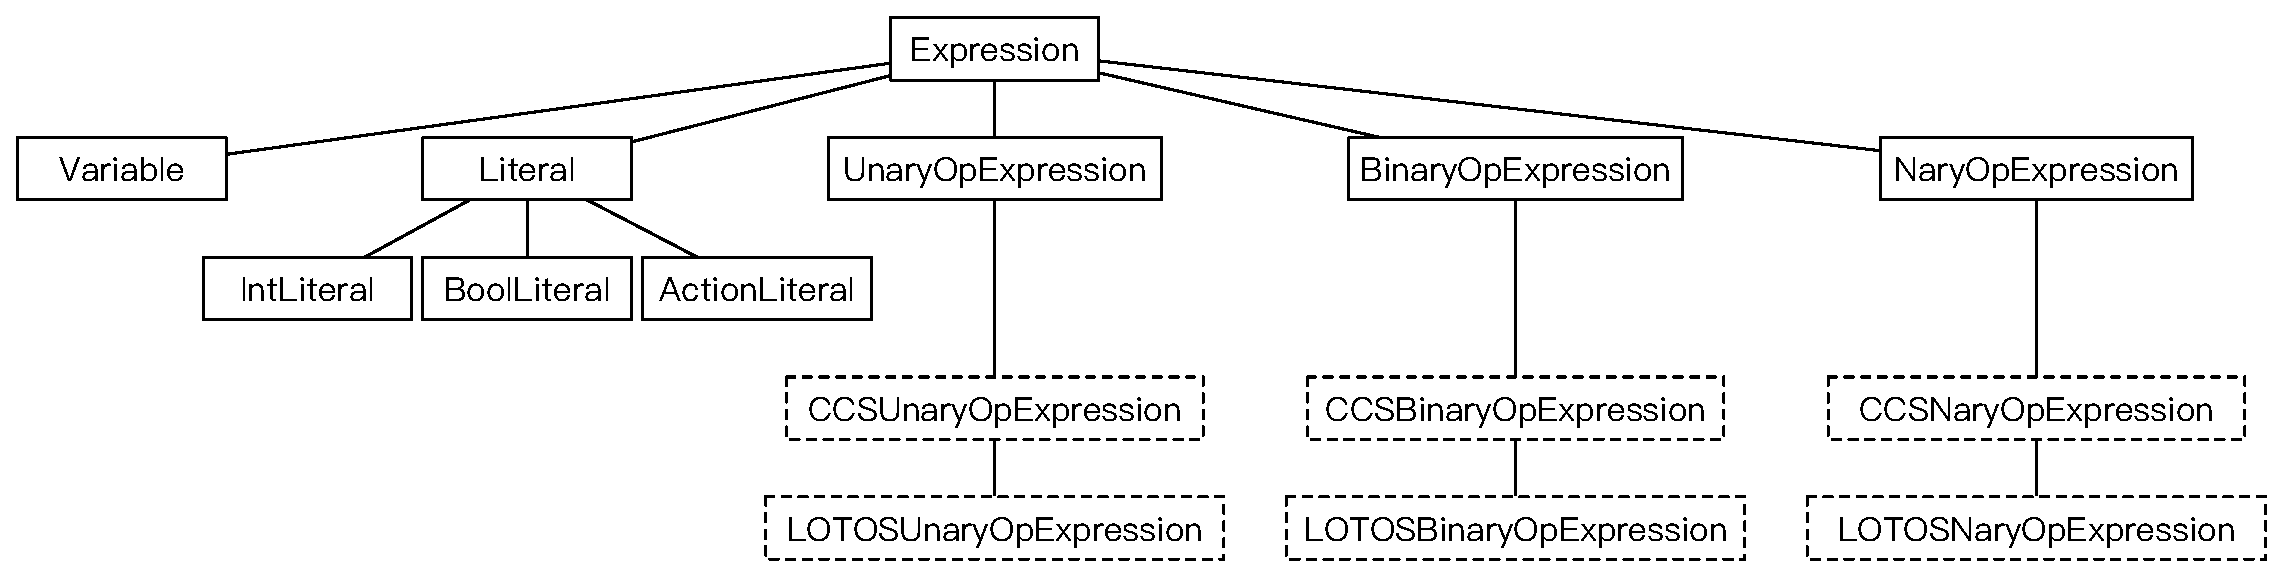
\includegraphics[width=\linewidth]{XFIG/Expression}
%  \caption{The architecture of Expression class}  \label{schema:expression-pnets}
%\end{figure}

%\TODO{give an example of user-defined sorts/operators, and tell that
%  you will give it's translation into Z3 in section 5.4}

% \TODO{To be move / replace by Xudong}

%\subsection{Computing and using open automata}
%In this section we present an algorithm to construct the open
%automaton representing the behavior of an open pNet, and show
%under which conditions this automaton is finite.
%
%\begin{alg}[behavioral semantics of open pNets: Sketch]
%This is a standard residual algorithm over a set of open-automaton
%states, but where transitions are open transitions
%constructively ``proven'' by deduction trees.
%
%1) Start with a set of unexplored states containing the initial state
%of the automaton, and an empty set of explored states.
%
%2) While there are unexplored states:
%
%2a) pick one state from the unexplored set and add it to the explored
%set. From this state
%build all possible deduction trees by application of the structural
%rules Tr1 and Tr2, using all applicable combinations
%of synchronization vectors.
%
%2b) For each deduction trees, extract the resulting
%open-transition.
%Its predicate is checked (using Z3) for  satisfiability. If it is
%unsatisfiable, the resulting OT is discarded. This will minimize the
%number of resulting transitions. 
%
%2c) For each open-transition,  add the transition in the outgoing transitions of
%the current state, and add the
%resulting state in the unexplored set if it is not already in the
%explored set.
%
%3) Finally a reachability check could potentially
%prune the state space.
%
%\end{alg}

%% \TODO{ERIC: after we move / replace Algoriithm 1, this will not make sense any longer. I will replace it with a more informal paragraph, in section 5}

%% To have some practical interest, it is important to know when this
%% algorithm terminates. The following theorem shows that an open-pNet
%% with finite synchronization sets, finitely many leaves and
%% holes, and each pLTS at leaves having a finite number of states and
%% (symbolic) transitions, has a finite automaton. The proof can be found
%% in \cite{henrio:Forte2016}. 
 

%% \begin{theorem}[Finiteness of open-automata.]\\
%% Given an open pNet $\mylangle \overline{\pNet},\overline{S}, \symb{SV}_k^{k\in K}\myrangle$ with leaves $pLTS_i^{i\in L}$ and holes $Hole_j^{j\in
%%   J}$, if the sets $L$ and $J$ are finite, if the synchronization vectors of all pNets 
%%   included in  $\mylangle \overline{\pNet},\overline{S}, \symb{SV}_k^{k\in K}\myrangle$ 
%%   are finite, and if
%% $\forall i \in L.\, finite{(states(pLTS_i))} \text{ and } pLTS_i$
%% has a finite number of state variables, then Algorithm 1 terminates
%% and produces an open automaton 
%% $\mathcal{T}$ with finitely many states and transitions.


% Given an open pNet $\mylangle \overline{\pNet},\overline{S}, \symb{SV}_k^{k\in
%     K}\myrangle$ with leaves $pLTS_i^{i\in L}$ and holes $Hole_j^{j\in
%   J}$,
% build its semantics as in algorithm 1.

% We have:

% $$ finite{(L)} \land finite{(J)} \land \forall i \in L finite{(\{s_i\})}
%   \to finite{(\mathcal{T})}$$
% \end{theorem}

\section{Implementation}
\label{section:implementation}
The VerCors platform uses pNets as the intermediate language
for some high-level language or graphical formalism to be translated
into both input for a model-checker and for generating executable code
automatically \cite{HKM-FASE16}.
We have extended the pNet API in VerCors to deal with open pNets, and
also to specify the structure of action algebras. 

In this section we describe the algorithm implementing the pNet
semantics, the interaction with the Z3 SMT solver, and we show the
result on our  example.

%\begin{algorithm}
%\caption{Open Automaton Generation}
%\begin{algorithmic}[1]
%
%\State Initialize sets $U$, $E$ for unexplored/explored global states
%$U$, $L$ for result OTs;
%\While{!isEmpty(U)}
%	\State Chose a global state $S$ in $U$; recursively applying Tr1 or Tr2 on the root node;
%	\If{Subnet is a pLTS}
%                \State Get the local state of the pLTS $s$ from $S$;
%		\For{each transition $tr$ starting from $s$} Apply Tr1
%			\State Build the corresponding
%                        $OT$; store $OT$ in $L$; 
%                 \EndFor
%	\EndIf
%	\If{Subnet is a pNet}
%		\For{each $sv \in SV$} Apply Tr2
%			\State Invoke $Combining()$ to generate the
%                        combination of sub-transitions, $Matching()$
%                        to match the combination with the $sv$; Store the result OTs in $L$; 
%		\EndFor
%	\EndIf
%	\For{each target global state $T$ from $OT \in L$}
%		\IfThen{$(!U.contains(T))\ \&\&\ (!E.contains(T))$}{Add $T$ into the $U$;}
%	\EndFor
%\EndWhile
%\State Prune the open transitions in $L$ using the SMT solver;
%\State \Return $L$;
%
%\end{algorithmic}  
%\end{algorithm}

\begin{algorithm}
\caption{Open Automaton Generation}
\begin{algorithmic}[1]
\Require The pNet node P.
\State Initialize sets $U$, $E$ for unexplored/explored global states, $L$ for result OTs;
\While{!isEmpty(U)}
	\State Chose $S$ in $U$;
	\State OT = MakeTransitions(P, S);
        \State Store $OT$ in $L$; 
	\For{each target global state $T$ from $OT \in L$}
		\IfThen{$(!U.contains(T))\ \&\&\ (!E.contains(T))$}{Add $T$ into the $U$;}
	\EndFor
\EndWhile
\State Prune the open transitions in $L$ using the SMT solver;
\State \Return $L$;

\end{algorithmic}  
\end{algorithm}

\begin{algorithm}
\caption{MakeTransitions()}
\begin{algorithmic}[1]
\Require The pNet node P; The start global state S.
\State Initialize a list $l$, $L$ for sub-transitions/transitions.
	\For{each Subnet in P}
	\\ ~~~ $\setminus \setminus$ Recursively applying Tr1 or Tr2 on the sub-nodes.
                \State Store MakeTransitions(Subnet, S) in $l$;
	\EndFor
	\For{each $sv \in SV$}
		\State $comb = Combining(l)$;
                 \State $ot = Matching(sv, comb, hole, v)$;
                 \State Store $ot$ in $L$; 
	\EndFor
\State \Return $L$;
\end{algorithmic}  
\end{algorithm}

\subsection{The Generation of Open Automata}

\QIN{
We have already have the sketch of computing the open automata \cite{???}.
While in our implementation we does not build explicitly a proof tree for every open transition.
Instead, we repeat applying the Tr1 or Tr2 to generate the sub-transitions.
Tr1 is applied on the leaf (pLTS) simply take the pLTS transitions through the given start state and add the predicate in pNet to generate the open transition.
When applying Tr2 we use two methods, combining and matching, to generate the new predicate of the open transitions in a hierarchical manner
as in this case the composition the subnets brings more constraints for synchronizing behaviors. 
Beside the new generated predicate, the predicates from the subnets are also added as a conjunction with those new predicates.
}

%Algorithm 1 shows the main structure of the algorithm: 
%the computation repeats applying Tr1 and Tr2 to build all possible
%combinations of behaviors of pLTS and Holes, through all possible
%synchronisation vectors. The resulting open transitions are checked
%for satisfiability by the SMT solver.

%From these, we compute
%the open automaton of an open pNet. We explain here our main
%implementation choices.
%:
%\begin{itemize}
%  \item Steps 2a-2b are merged, applying Tr2 from the
%premisses OTs from subnets to generate OTs without
%explicitely constructing the deduction tree.
%  \item We define a general naming schema for implementing the fresh 
%and clone functions with more structure than a simple global name
%generator. It ensures unicity, but builds names
%readable enough for debugging purpose.
%  \item Besides that, we also have designed a management of state variables and
%    assignments throughout the whole computation.
%%%   \item Satisfiability check is done only at
%%% top level of the open-transition construction. An alternative would be
%%% to submit the satisfiability check to the SMT solver at each level of
%%% the hierarchical OT construction, potentially reducing the overall number of
%%% combinations. But the submission to the SMT engine is costly, and more
%%% complexity analysis is required before deciding if this would be
%%% worthwhile. 
%\end{itemize}
%
%In the following sections, we detail:
%\begin{itemize}
%\item The structure of fresh variable names.
%\item The details of the implementation for step 2a-2b, refined into:
%  \subitem combining all possibilities of subnets activity/inactivity,
%  \subitem matching each combination with synchronization vectors.
%\item Management of local variables of pLTSs.
%\item Pruning unsatisfiable OTs using the Z3 SMT solver.
%\end{itemize}

%\TODO{I have not yet been in details through the next section, but we
%  need to shorten them...}

% \TODO{Xudong: move here a (new version) of the alogorithm loplevel sketch}
% \QIN{[Move to the head of Section 5.]}

%% \QIN{
%% The detail about the application of the Tr1 and Tr2 have not considered in the sketch, but it is an  
%% important part in the implementation of open transition generation. 
%% Each time we apply Tr1, there is not too much predicate terms, so do the other parameters, needed 
%% to be generated. 
%% When it comes to applying Tr2, the computation becomes complicated because it doing some composition of the subnets.
%% }

%\paragraph{Combining and Matching using TR2}
%Our implementation does not build explicitly the proof trees for each
%open transition, but instead : [Combining] enumerate all possible combinations of
%pLTS transition (using TR1) and each synchronization vector choice
%(TR2); [Matching] build the corresponding transition, and in particular
%its predicate, in a hierarchical manner.
%Each time we apply Tr2, we build a predicate as a conjunction of two
%parts. The first part, which is the simpler one, composes the
%predicate from the 
%subnets and the guard from transitions in sub-pLTS or synchronization
%vectors. The second part is the conjunction of equations generated
%during matching the subnets' behaviors with the synchronization
%vectors. 

%Note that it is simple to collect required terms in the first
%part while in the second part we need to find out all the possible
%conjunction forms. We present here a algorithm divided in two
%step. Combining enumerates all the possible combinations of the
%working status. Matching synchronizes the subnets according to
%synchronization vectors to generate possible predicates.  
 
%Combining is to generate all the possible matchings of the subnets' OTs (open transitions). The result list of the matched tuples called *combination*.
% 1. Initialize the result list of OT tuples.
% 2. Get one list of OTs. It's same as get OTs of one subnet.
% 3. Add *null* into the list, it means this subnet does not work this time.
% 4. Combine the rest subnets' OTs. Get the combination of the rest OTs.
% 5. If there are OTs of the chosen list not be chosen, choose one OT.
%      1. If there are tuples of the combination not be chosen, choose one tuple.
%          1. Add the chosen OT into the tuple.
%          2. Add the tuple into the result list, then do the recursion.
% 6. Return the result list.

%We first conduct combining. For each subnet, we enumerate all the
%possible cases of its working status. The result action of a pLTS or a
%pNet is the external action of the node shows the working status of
%it.
%
%For holes, their behavior is unspecified, it doesn't have an exact
%external presentation of action. We only give an action variable to each hole
%and treat it as hole behavior to suppose working status of the
%hole.
%% Here should have a constraint that this variable belongs to the sort of hole.
%In every case, the hole behaviors are unchanged, so we
%only make the combinations of subnets' open transitions. 
%
%Algorithm 1 shows the combining algorithm for enumerating all the possible combinations of open transitions. The algorithm initializes an empty list $L_C$. Dealing with the list $TR$ containing several sets of open transitions from different subnets, the algorithm only chooses one of sets $L_{ot}$ and does combining on the remaining part of $TR$ recursively then get a partial result of combining, $L'_C$. Since there could exist the case that the subnet is not working, a $null$ is added into the $L_{ot}$ to represent it. We get much more combinations after combining $ot$ from $L_{ot}$ with the partial result. 

%\begin{algorithm}
%\caption{Combining}
%\begin{algorithmic}[1]
%
%%\Require The list $TR$ of the open transition sets of the subnets. 
%%\Ensure The list of all the possible combinations of open transitions $L_C$.
%\State Initialize an empty combination list $L_C$;
%\State Extract a list of open transitions $L_{ot}$ from $TR$;
%\State Add $null$ to $L_{ot}$;
%\State Get the combinations $L'_C$ of the $TR$;
%\For{each $ot \in L_{ot}$}
%	\For{each $C' \in L'_C$}
%		\State Add $ot$ into $C'$ to get a new tuple $C$;
%		\State Add $C$ into $L_C$;
%	\EndFor
%\EndFor 
%\State \Return $L_C$;
%
%\end{algorithmic}  
%\end{algorithm}

\paragraph{Combining:}
\QIN{
The combining method enumerate all the possible status of the subnets.
The result of the method hence call the combination as it present as all the possible combinations of their open transitions.
Assume that there is a collection of $n$ subnets $L = {s_1, s_2, ..., s_n}$, if we notate $ot$ to be the set of open transitions of the subnet $s$ and $\eta$ means the subnet is not involved. 
Then the combination $\texttt{COMB}$, a set of n-tuples, can be computed as an outer product of sets : 
\[\texttt{COMB} : (\eta\cup ot_1) \times (\eta\cup ot_2)\times ... \times (\eta\cup ot_n) .\]
}
%Algorithm 2 shows the combining algorithm for enumerating all possible
%working status combinations from subnets. Dealing with a list $TR$
%containing  sets of open transitions from different subnets,
%the algorithm choses one of sets $L_{ot}$ and does combining on the
%remaining part of $TR$ recursively. The case when a subnet is not working is
%managed by adding a $null$ into the $L_{ot}$.


% Mixing is to match the combination of the subnets' open transitions, hole behaviors and result action with the SV (synchronization vector) to generate the possible predicates of the OT (open transition). At the same time, other parameters of the OT (global state, subnets' transitions, result action...) are also generated. Then the possible OTs of the pNet can be achieved. 
% 1. Initialize the combination through the method *combineOpenTransitions( )*.
% 2. Initialize the result list.
% 3. Get the number of subnets and holes. They are used to decide how many element of the SV should be matched with them.
% 4. For all tuples of the combination.
%      1. Invoke the *clone( )* method to generate the fresh SV.
%      2. Match the elements of the tuple with the elements of the SV. If there is a *null* matched with a *not null* action, filter this matching. Add the result expression and the predicate of the subnets into the predicate. Generate the target global state correspondingly.
%      3. Match the hole behaviors with the elements of the SV. The hole behavior could be *null*. Add the result expression into the predicate.
%      4. Match the result action with the result action of SV. Add the result expression into the predicate.
%      5. Add the predicate into the OT. Store the OT in the result list.  
% 5. Return the result list of all the possible OTs.


%We now come to the matching using combinations from the previous step, together with hole behaviors and the result action, to match with the synchronization vectors. 
%
%Algorithm 2 shows the algorithm matches combination $L_C$, hole
%behaviors $B$ with synchronization vectors $SV$. Remember variables
%inside a synchronization vector are consider local to the vector; so every time we choose a synchronization vector $sv$ from $SV$ for matching, we clone it and use the cloned one $sv'$. We use the definition declared before to construct all the possible predicates but the algorithm has not checked the correctness of these predicates. 
%
%There is one mismatch case we can easily detect here, that is its
%working status:
%At any time an action $e_1$ matching with an element $e_2$ from
%synchronization vector, the pair $(e_1, e_2)$ must be checked: if both
%$e_1$ and $e_2$ are $null$ or $not\ null$, then it continues to
%generate a new term of predicate. Otherwise, it is intuitive that the
%working status coming from the subnet $e_1$ is different from what
%asked by the synchronization vector $e_2$, then this case is filtered
%out.

%\begin{algorithm}
%\caption{Matching}
%\begin{algorithmic}[1]
%%\Require 
%%The combination of subnets' open transitions $L_C$;
%%The behaviors of the holes $B$;
%%The set of synchronization vectors $SV$.
%%\Ensure 
%%The list of all the possible open transitions generated $L_{ot}$.
%\State Initial an empty result list $L_{ot}$;
%\For{each $C \in L_C$}
%	\For{each $sv \in SV$}
%		\State Clone the $sv$, the result is $sv'$;
%		\State Generate the fresh result action $ra$;
%		\State Combine $C, B, ra$ as a new vector $v$;
%		\For{each $(e_1 \in v )\&\& (e_2 \in sv')$}
%			\If{$(e_1\ is\ null\ \&\&\ e_2\ is\ not\ null)\ ||\ (e_1\ is\ not\ null\ \&\&\ e_2\ is\ null)$} 
%			\State Skip;
%			\Else ~ Add $(e_1 = e_2)$ into the $Pred$;
%			\EndIf
%		\EndFor
%		\State Generate the result open transition $ot$ with $Pred$;
%		\State Add the $ot$ into $L_{ot}$;
%	\EndFor
%\EndFor 
%\State \Return $L_{ot}$;
%
%\end{algorithmic} 
%\end{algorithm}

\paragraph{Matching:} 
\QIN{$Given a synchronization vector ~ SV_k\in SV = (a'_i)^{i\in I} (b'_j)^{j\in J}\rightarrow v' , G_k , k\in K$, and a tuple
$C_n\in \texttt{COMB} = {(v_i)}^{i\in I} , n\in N$ where $K$ and $N$ are the indices of the set elements.
As the behavior of subnets should match with the synchronization vector to compose the subnets.
The matching method tries matching $SV_k$ and $C_n$ to generate the predicates.
According to the definition of predicate, the hole behaviors $Hole$ and result action $v$ are also involved. 
}

\QIN{
$$Matching(SV_k, C_n, Hole, v) = 
\begin{array}{l}
\forall {(a'_i)}^{i\in I},
{(b'_j)}^{j\in J},v'.
\\
v_i=a'_i\land \, b_j=b'_j \land v=v' \land G_k
\end{array}$$
which is exactly the new part of predicate for one possible result.
}
%Algorithm 3 shows the algorithm matches
%combination $L_C$, hole behaviors $B$ with synchronization vectors
%$SV$ according to the definition of the predicate declared before. We
%clone the $sv$ using the fresh function to generate a new $sv'$ with
%fresh variables.The mismatch on working status is easy to detect so we
%filter them in the algorithm through checking the matching elements
%$e_1$ and $e_2$. 
%Then we build the resulting open transition. Satisfiability of the
%predicate is not checked at this level, but only later, at the
%toplevel of the pNet.

\paragraph{Filtering:} 

\subsection{Management of state variable assignments}
%The pLTS contains some variables in each of its states (state
%variables), or just as global states of the pLTS (global variables).
%Both can be assigned in the pLTS transitions.
%The algorithm composing assignments from subnets is different from the
%generation of predicates. 
%%When applying Tr1, we just keep the
%%assignments in the Post of the open transition. And when it comes to
%%Tr2, Post is the union of the assignments propagate from the
%%subnets. 
%The assignments provide value of the variables in
%predicates. There is usually not only one assignment for a state variable as
%several incoming transitions of a state can perform different
%assignments on the same variable. The values of the
%variables are necessary for checking satisfiability of the open
%transitions together with predicates, miss of them may drop the
%unsatisfiable results. In order to avoid such mistakes, the algorithm
%manages the variables together with a list.
%
%The list we used contains triples $<v,\ S, \ AssignRH>$ set for each pLTS to record
%the information of both state and global variables of the pLTS where $v$ is the variable in pLTS, $S$ is its owner state and $AssignRH$ is a list of expressions over other variables in the right hand side of assignments of $v$. The $S$ can be $null$ in the record triple, it means the variable is global in the pLTS belonging to all the states. 
%%So it should be noted that the changing of the value of the global state variable every time a transition is conducted. $AssignRH$ is the collection of all the possible expressions coming from the the right hand side of assignments. It keeps the information of the assignments for each variable. 
%We update the list of record triples every time Tr1 is applied, adding the right side of the assignments into corresponding expression lists. So the list keeps the all the assignments in the pLTS. Then we can track all the possible value of the variables when computing open transitions. 
%The initial value of the state variable is also seen as an assignment
%for that variable. We must give a initial value to the global state
%variable or there will be some problem in the start state. However, we
%sometimes don't give initial values to the state variables (except the
%global variables) as their initial values are decided by their first
%assignments. Checking whether each variable is initialized before
%being used is a separated problem, that should be done before starting
%our algorithm.

In a pLTS, there may be several incoming transitions of some states
that assign potentially different values to a state variable.
To handle such cases, the algorithm manages the variables together
with a list for each pLTS.
The list we used contains several triples <$v$, $S$, $AssignRH$> 
where $v$ is the variable in pLTS, $S$ is its owner state and
$AssignRH$ is a list of expressions over other variables in the right
hand side of assignments of $v$.
As a pragmatic extension to the formal definition, we also manage
``global variables'', defined in all states of the pLTS.

%There are some assignment on the variables in each of states of the pLTS (state variables), or just as global states of it (global variables). There is usually not only one assignment for a state variable, miss of them may drop the unsatisfiable results. In order to avoid such mistakes, 


%% \QIN{
%% The list we used contains several triples <$v$, $S$, $AssignRH$> to
%% record the information of both state and global variables of the pLTS,
%% where $v$ is the variable in pLTS, $S$ is its owner state and
%% $AssignRH$ is a list of expressions over other variables in the right
%% hand side of assignments of $v$. It means the variable is global in
%% the pLTS belonging to all the states, if $S$ is $null$. We update the
%% list of record triples every time Tr1 is applied. Then we can track
%% all the possible (symbolic) value of the variables when computing open transitions.
%% }

\subsection{Pruning the unsatisfiable results}
\label{section:pruning}
%We have used a brute-force method to generate all the possible open
%transitions in the open automaton. It obviously contains some of
%unsatisfiability in the open transitions. In
%Fig~\ref{schema:unsat-ot}, we display an unsatisfiable open transition
%from the result of the CCS running example. It shows the case that the
%top level transmits out the action from the PN2, formula $a.P$, as
%this time only PN2 is working and C1 is performing action $a$ when
%hole $P$ is also working. When matching this case against the second
%synchronization 
%vector of PN2, transmitting the behavior from hole $P$ to the higher
%level, is used while it is obviously violate the guard of the
%vector. So we can easily find the contradiction between the generated
%predicate term $ra:152:1=l \!\land\! a=:ra:152:1$ and the guard
%composed into the predicate $a \neq l$.

\begin{figure}[h]
%$\begin{array}{@{}r@{}l@{}}
%%{s0---a-->s1},   {---:hb:15:2-->},   (:ra:15:2 = act:sva:1:3)/\(:ra:152:1 = l)/\(a = :ra:152:1)/\(l!= a)/\(:hb:15:2 = y:sva:15:2)/\(:ra:15:2 = y:sva:15:2)/\(y:sva:15:2 != l)/\(:ra:1:3 = act:sva:1:3)
%    ot  = &\openrule{\{0 \xrightarrow{a} 1\}, ~~\{\xrightarrow{:hb:15:2}\}, ~~:ra:15:2=act:sva:1:3 \\
%    \OTland:ra:152:1=l \OTland a=:ra:152:1 \OTland a \neq l \OTland :hb:15:2 = y:sva:15:2 \\
%    \OTland :ra:15:2 = y:sva:15:2  \OTland y:sva:15:2 \neq l \OTland :ra:1:3 = act:sva:1:3}
%    {\ostate{00} \xrightarrow{:ra:1:3} \ostate{10}}\\
%  \end{array}$
%\caption{One of the unsatisfiable open transitions in CCS running example}  \label{schema:unsat-ot}
%\end{figure}

%{s0---delta-->s0},   {---:hb_P:12:1-->},   (:ra:11:1=l)/\(delta=:ra:11:1)/\(var_s0=0)/\(:hb_P:12:1=a1:sva_SV0:1:1)/\(:ra:1:1=a1:sva_SV0:1:1)/\(a1:sva_SV0:1:1!=delta(x)),   {var_s0 := 1}
$\begin{array}{@{}r@{}l@{}}
    ot  = &\openrule{\{0 \xrightarrow{\delta} 0\}, ~~\{\xrightarrow{:hb:12:1}\}, ~~\OTvar{:ra:11:1}=l \OTland \delta=\OTvar{:ra:11:1} \OTland \OTvar{s0}=0 \\
     \OTland \OTvar{:hb:12:1}=\OTvar{a1:sva:1:1} \OTland \OTvar{:ra:1:1}=\OTvar{a1:sva:1:1} \OTland \OTvar{a1:sva:1:1} \neq \delta(x), ~~\{\OTvar{s0} \leftarrow 1\}}
    {\ostate{00} \xrightarrow{\OTvar{:ra:1:1}} \ostate{00}}\\
  \end{array}$
\caption{One of the unsatisfiable open transitions in LOTOS running example}  \label{schema:unsat-ot}
\end{figure}

We use a brute-force method to generate all the possible open
transitions in the open automaton, using all possible combinations of
synchronization vectors. Naturally this builds some transitions where
the predicates express incompatible constraints. Even if having an
unsatisfiable (symbolic) transition in the open automaton would not be incorrect,
we want to check them for satisfiability, and reduce the number of
transitions and states in the automaton.
In Fig.~\ref{schema:unsat-ot}, we display an example of an
unsatisfiable open transition 
from the result of our example. It shows the case where
the controller C1 wants to move the control from $P$ to $(acc(x);Q)$,
conducting a $\delta$ transition. However, a synchronization
vector is chosen that does not match with this action, and we can
easily find the contradiction in the 
generated predicate term ``$\OTvar{:ra:11:1}=l \!\OTland\! \delta=\OTvar{:ra:11:1}$''. 

Checking satisfiability requires some symbolic computation
on the action expressions and the predicates, and this 
may depend on the specific theory of the action algebra. 
We use the SMT solver Z3 to check the predicate of the result open transitions, 
it will return whether the predicate is satisfiable or not.
The ``Modulo Theory'' part of SMT solvers is important here, so that
the solver can use specific properties of each action algebra.


\begin{figure}[t]
  %  \centerline{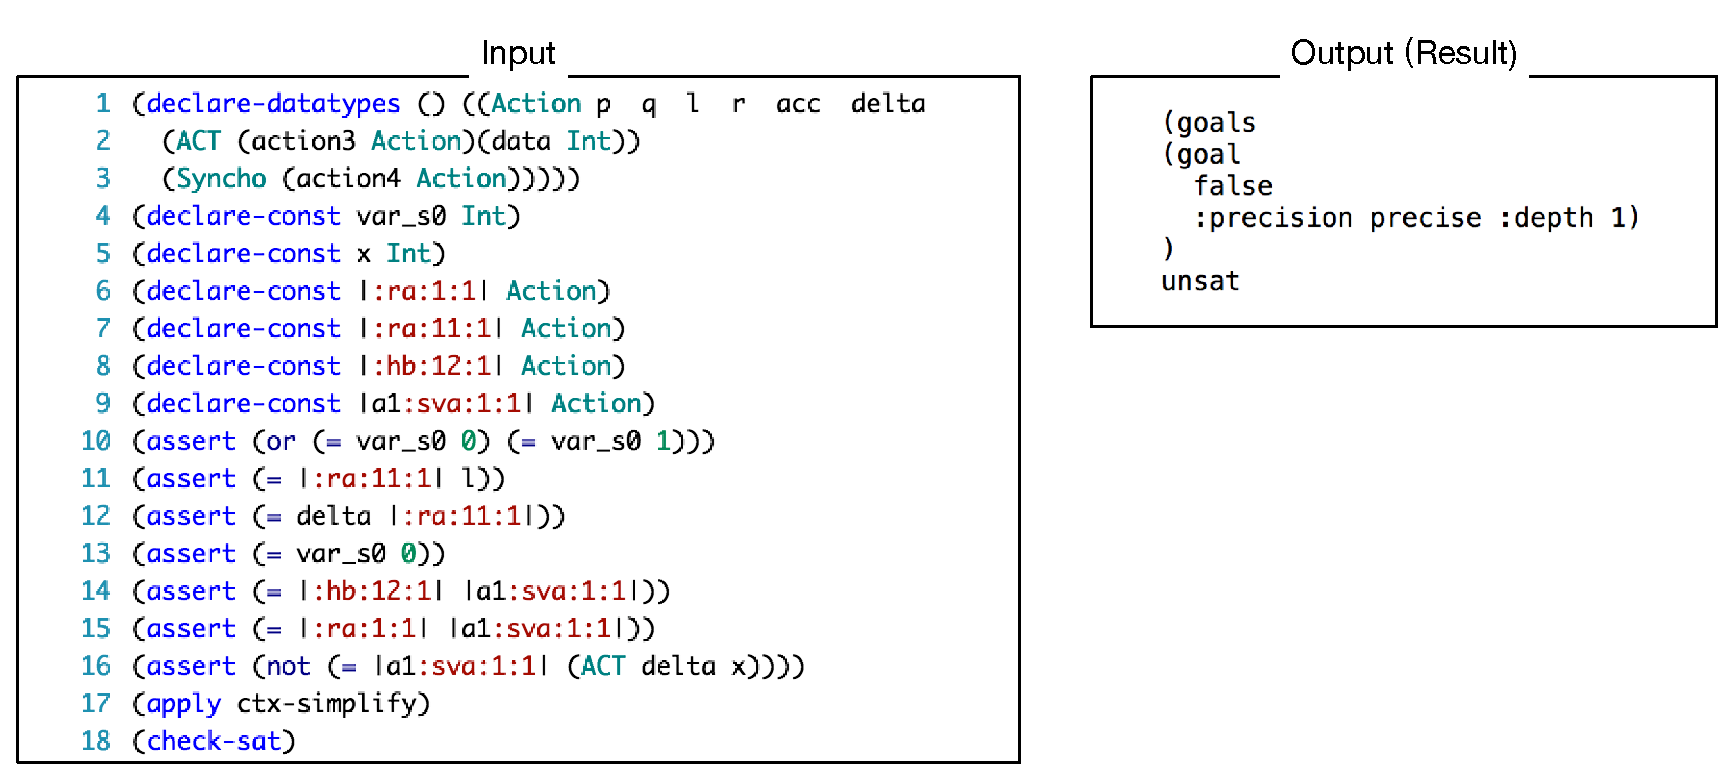
\includegraphics[width=12cm]{XFIG/SMTLIB2}}
    \centerline{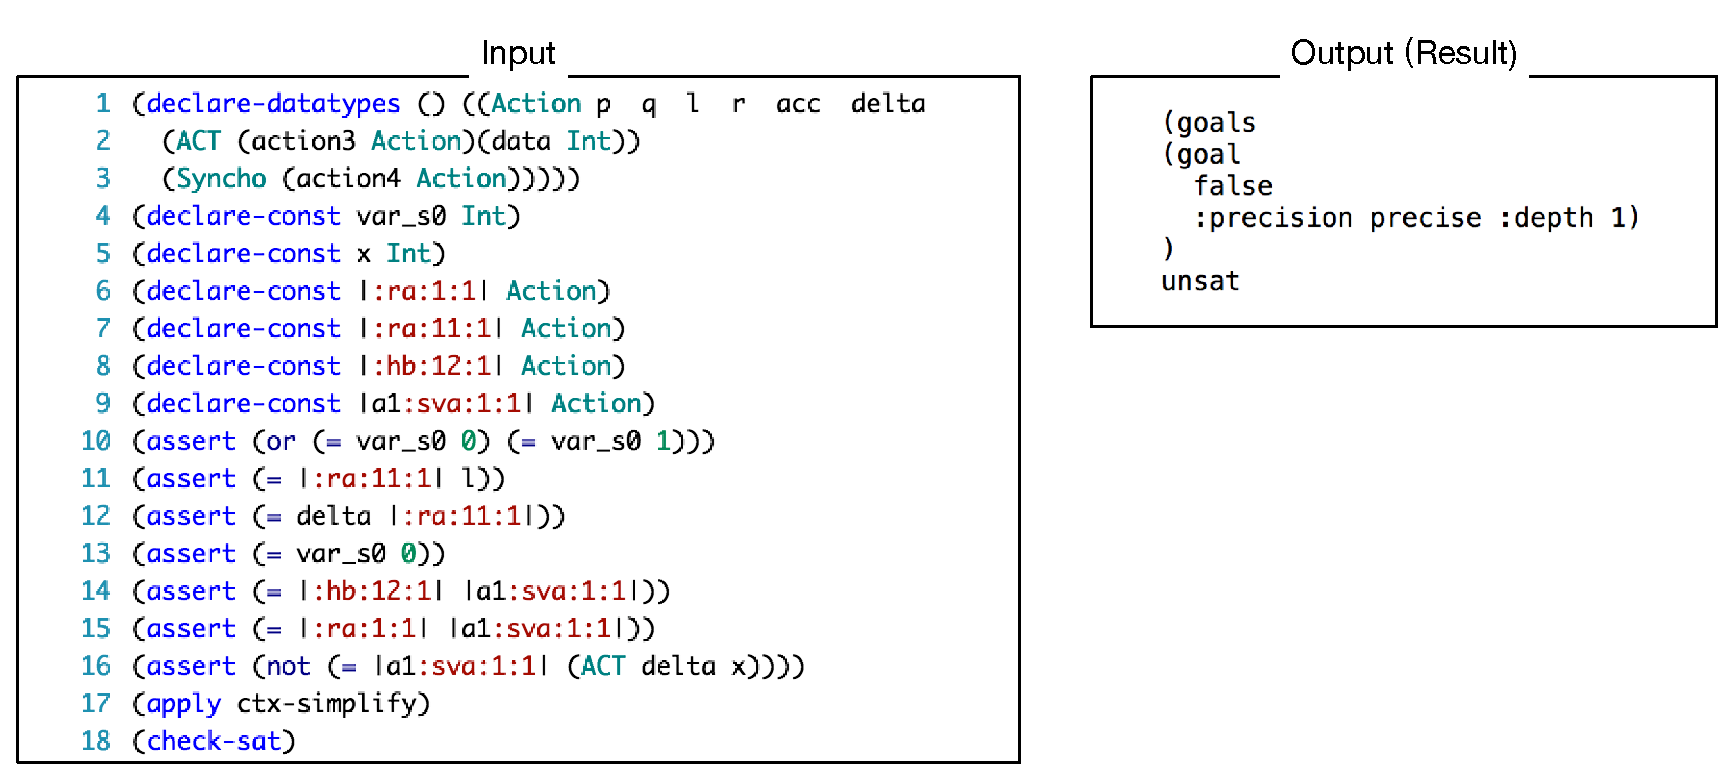
\includegraphics[width=\linewidth]{XFIG/SMTLIB2}}
  \caption{The input of the Z3 solver in SMT-LIB language and the output result}  \label{schema:smt-lib}
\end{figure}

%% \begin{figure}[t]
%%   \centerline{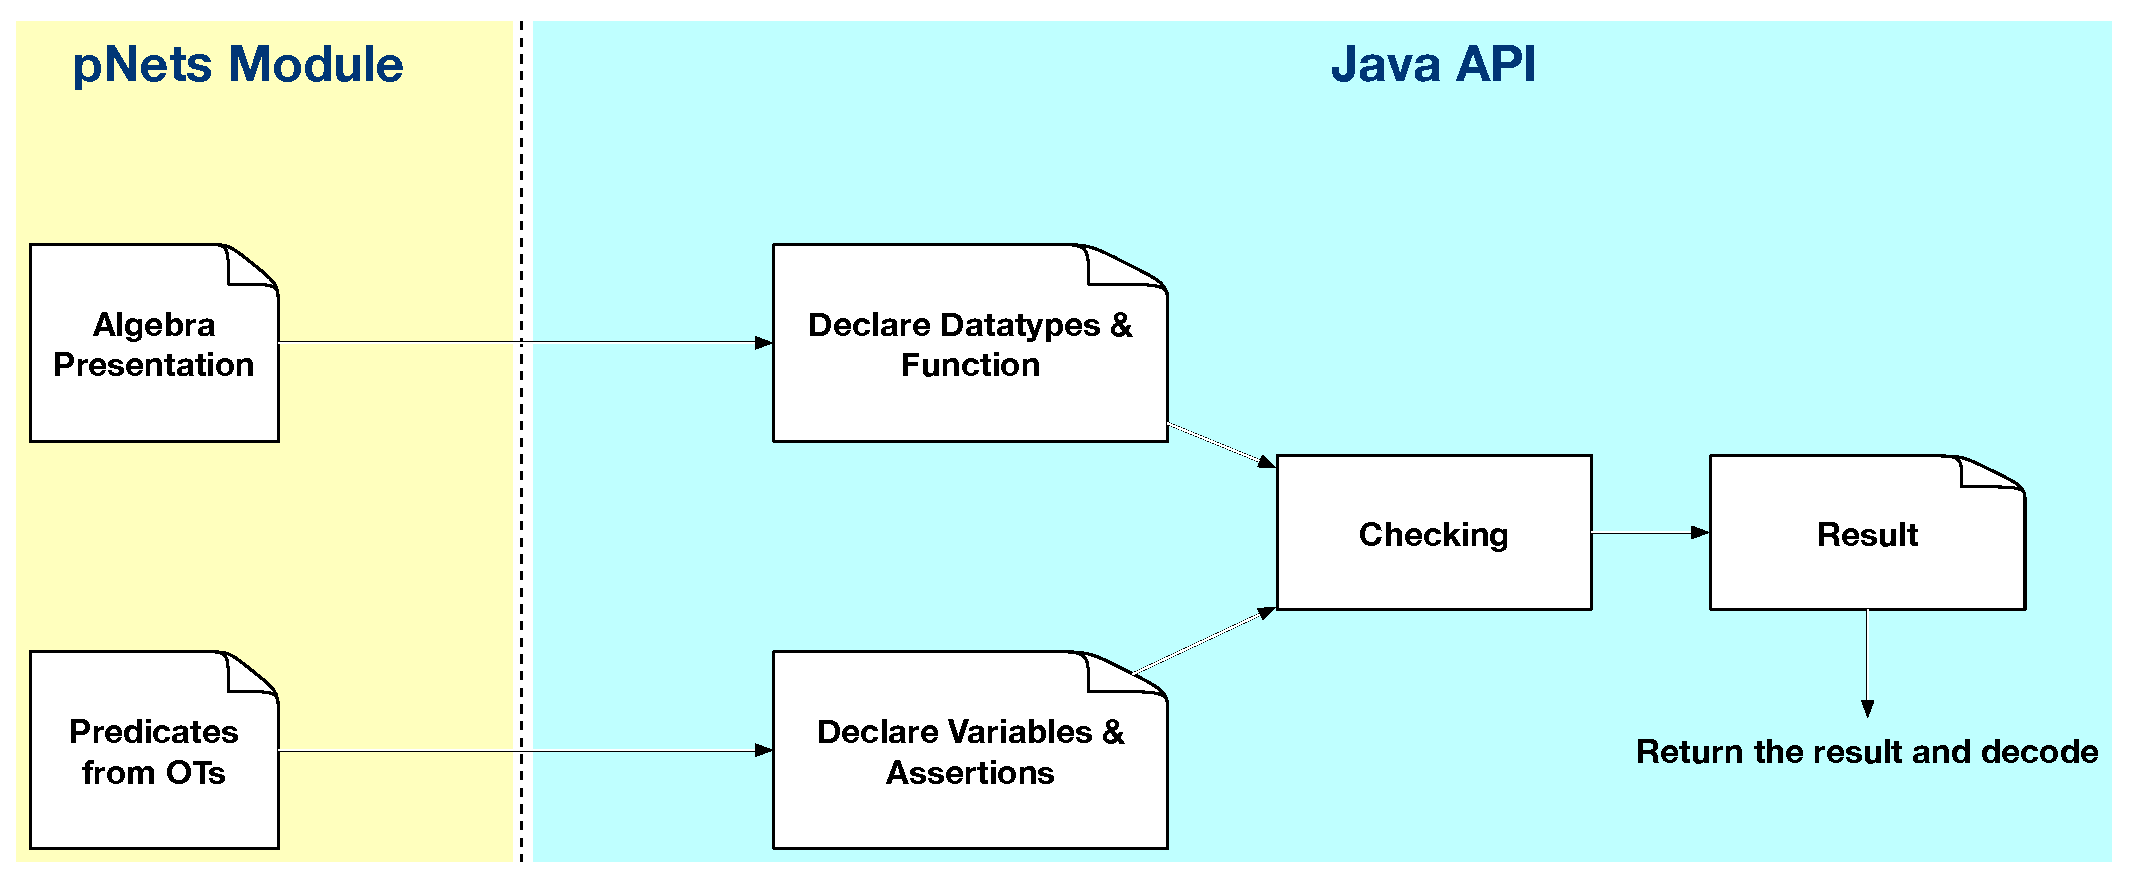
\includegraphics[width=10cm]{XFIG/Interaction}}
%%   \caption{The architecture of the interaction between pNet API and Z3}  \label{schema:interaction}
%% \end{figure}

\subsection{Translation to SMTlib}

\paragraph{Presentation of algebra}

\TODO{Improve this, inserting the main definition from the ``Checker'' document}
%% Open pNet framework provides us
%% with a model able to express the semantics of many different algebras
%% or languages. In particular,
As seen in section
\ref{section:pnets}, the \emph{term algebra} used to express the
action expressions and data parameters is left open in
the pNet definition.

So, for a given language, we now need to specify its data and action
domains, giving them an abstract syntax (sorts, constructors, operators,
and predicates). We call this a \emph{Presentation}.
We also define a concrete syntax, that will be used for
pretty-printing, but also for translating the presentation, and the
predicates, into Z3 syntax (see the ``declare-datatypes'' statement in
Fig~\ref{schema:smt-lib}). 

An algebra presentation contains:


\begin{itemize}
	\item Sorts: Constants sets of the algebra or types of the data
          and actions (integer and boolean sort are implicitly
          declared).  There \emph{must} be one sort for actions, and
          eventually others for the types of data
          parameters. In the LOTOS example, 
          we have the $Action$ sort: $\OTvar{Action = } \{ l, \delta,
          r, p, q, acc \} .$ 

	\item Operators:
          %Operators used to construct action expressions; they are
          constructors and predicates for data and action sorts. For
          instance, in our LOTOS example, we
          have a generic action constructor ``$ACT$'', taking as
          argument an action litteral and a data parameter, declared as:
          $\OTvar{ACT:}\OTvar{< Action, Data >} \rightarrow \OTvar{Action.}$, 
        \item Constants: The satisfiability solver need to know which
          actions in the pLTS behaviors are constants (like the $l$, $\delta$, 
          $r$ of the controllers in running example). 
          For a given pNet system, the sort $Action$ will include all
          these constants.
\end{itemize}

\paragraph{Interaction with Z3}
%\TODO{1. example input of Z3 in SMT-LIB.[DONE] 2. software architecture.[DONE]}
%There are several ways to interact with the Z3 solver. 
%It is possible to use Z3 interactively using the SMT-LIB
%(Python-based) language. 
From inside our algorithm code, we submit satisfiability requests to
Z3 using its JAVA API. Here for readability, we
show the Z3 code using its SMT-LIB input language. As an
example in
Fig~\ref{schema:smt-lib}, we show the input for checking the
transition of Fig.~\ref{schema:unsat-ot}. It contains the declaration
of the LOTOS action algebra types 
and constructors, then the declaration of variables, and finally the
predicate to be checked, encoded as a set of assertions.
%% Generally, some $datatypes$ are declared to input the sorts, while here
%% we only declare one $datatypes$ named $Action$ to involve all the
%% constant actions. Then we input the predicate of this open transition
%% in two parts: the variables contained in the predicate are declared
%% first, then the terms of predicate are inputed as $assertions$ one by
%% one. 
The result "unsat" in the output is just what we expected.   

%\TODO{edit the figure to make it smaller in height [DONE]}

%We present the architecture of the interaction with Z3 in
%Fig~\ref{schema:interaction}.
%For each OT generated at the toplevel of a pNet, the predicate must be
%submitted for satisfiability check to Z3. For that we need to
%translate into Z3 (Java-API) syntax, both the elements of the action
%algebra, and the predicates itself, including the encoding of the
%variable assignments (the Post part).
%
%The $presentation$ of the action algebra
%is declared at the beginning of the algorithm as the $sorts$ and the
%$operators$ will be used throughout the whole algorithm. It is
%translated into $datatypes$ and $functions$ then submitted to the Z3
%at the same time. Each candidate predicate will then be translated
%into $assertions$ before submitted to Z3 after the algorithm
%computing out all the possible open transitions, they act as
%intermediate results there. Together with the $datatypes$ and
%$functions$, the $assertions$ are used to check the satisfiability of
%the predicate in Z3.

To build the input submitted to Z3 for each OT,
we translate the algebra $presentation$, the predicates and the
variable assignments (the Post part) into Z3 (Java-API) syntax.
% The $presentation$ and the predicates are translated separately. 

\paragraph{Translation of Action algebra presentation}
\TODO{Exerpt of the formalisation}
The $datatypes$ are declared according to the $sorts$ the users
declared in the $presentation$. If the return type of the $functions$
is one of the $datatypes$, we add this $function$ to the $datatypes$ declaration.
So when we declare the operator ACT we illustrated in section 4.1, it
will be just declared together with the constants like :\\
\centerline{$\OTvar{(ACT\ (action3\ Action)(data\ Int))}$}

The $functions$ can also be declared independently, it usually applies to functions returning integer or boolean, in the format like:\\
\centerline{$\OTvar{(declare\text{-}fun\ MAX\ (Int\ Int)\ Int)}$}

%Although in Fig~\ref{schema:smt-lib} we have not declared $functions$ outside of $datatypes$, there still exists $functions$ declared independently. The input and output types of the $function$ are also determined by the construct of the  $operators$ in the presentation. For example, we define a new operator to present the equation between two actions in LOTOS example $\text{EQUAL}$ in the format likes:
%
%\[EQUAL: \quad < Action , Action > \rightarrow Bool .\]
%
%It will be translated into the Z3 statement: 
%
%\[\text{(declare-fun\ EQUAL\ (Action\ Action)\ Bool) .}\]

\paragraph{Translating assignments into predicate terms}
\TODO{Exerpt of the formalisation}

%The assignments are also taken into account when checking the
%satisfiability of the open transitions as they represent the value of
%the variables involved in an OT. In order to do that, we employs a
%translation from assignments into term of predicates. The assignments
%required to be translated are only those belong to the variables
%contain in the start states of the open transitions. The assignments
%are represented as equations between the variables and the expressions
%on the right side of assignment. For the assignments of the same
%variable, we do not figure out which state is the precursor of current
%state, we keep all these possible equations instead, and generate the
%disjunction of these equations. The state could always move to the
%target state if there exists one of the values of its variable
%satisfies the guard.
%%\TODO{It won't matter the variable of the next state
%%except that the right hand side expression contain its variables. This
%%is a problem left to be solved in our future work. WHICH PROBLEM ?}
%After that, for the assignments of the different variables, we generate a conjunction of them. This way we obtain a new term of the predicate involving assignments of the variables.

State-variable assignments are also treated as a part of the
predicates when checking the satisfiability. % Here we need conduct some
% translations,
For each assignement in a $\Post$ predicate, such as $\{s_0 \leftarrow 1\}$ in section
~\ref{section:op-semantics}, we translate it into an equation
$s_0=1$. For several assignments of the same variable in the same state,
we generate the disjunction of 
these equations. Correspondingly, we generate a conjunction for the
assignments from different variables. 


\paragraph{Checking satisfiability}

% We check the satisfiability of open transitions on the top level of
% the pNet, treating these open transitions as the intermediate result
% of the algorithm. After we get the intermediate results of open
% transitions, we check them one by one.
Here we declare first all the variables in the predicates, with their
sorts.
An example of syntax is::\\
\centerline{$\OTvar{(declare-const\ |:ra:1:1|\ Action)}$}

\noindent Then each term of the
predicate is an assertion in Z3, as an example, in the former
unsatisfiable result in Fig~\ref{schema:unsat-ot}, the contradiction is occurred in terms: \\
\centerline{$\OTvar{(:ra:11:1=l)} \OTland \OTvar{(delta=:ra:11:1)}$}\\
from which we generate the following two assertions:\\
\centerline{$\OTvar{(assert\ (=\ |:ra:11:1|\ l))\ \ \ (assert\ (=\ delta\ |:ra:11:1|))}$}

\noindent The predicate submitted to the Z3 also contains the
assignments encodings.
In the case of $ot_2$, it
gives the assertion:\\
\centerline{$\OTvar{assert (or (= var\_s0 0) (= var\_s0 01)))}$}

\subsection{Simplification of Predicates}

\subsection{Result of the running example}
\label{section:full-result}

\TODO{Update: we have 11 satisfiable OTs here}
Our tool builds 30 open
transitions, out of which 27 are detected unsatisfiable by Z3, we
get only 3 results left; the resulting open automaton is shown in
Fig. ~\ref{schema:lotos-result}, together with its open transitions.

The resulting open transitions represent all the
possible movements of the LOTOS example.
What can be observed is any actions of the process $P$ from the beginning, until $P$ performs a $\delta(x)$ and the value of
$x$ is transmitted to the $acc(x);Q$ giving out a silent action. Such behavior is performed by the $ot_1$ then $ot_2$. 
Then it keeps presenting the behavior of $Q$, as seen in $ot_3$. 
%The $ot_1$ transition means that the actions of the process $P$ could
%be transmitted out, until $P$ performs a $\delta(x)$ and the value of
%$x$ is transmitted, through transition
%$ot_2$. The other 3 open transitions shows the behaviors of the
%process $Q$ while the $ot_3$ and $ot_4$ won't be performed as the
%controller has already set the value $s_0$ to 1 in the previous
%action. 

\begin{figure}[t]
   \centerline{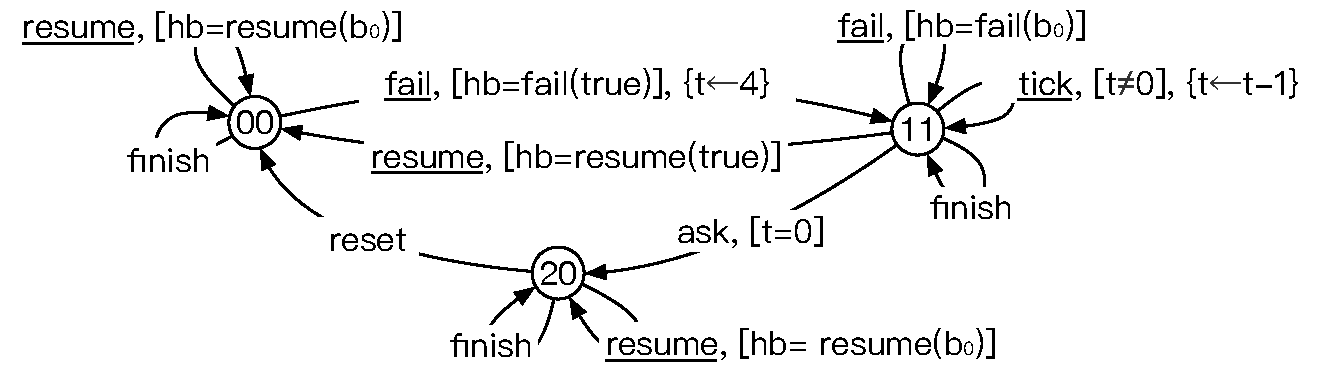
\includegraphics[width=12cm]{XFIG/BIPresult-ArchFailureTimerMax}}
   \caption{Open Automaton\TODO{syntax could be better...}}  \label{schema:resultOA}
 \end{figure}


\begin{figure}[h]
%  \centerline{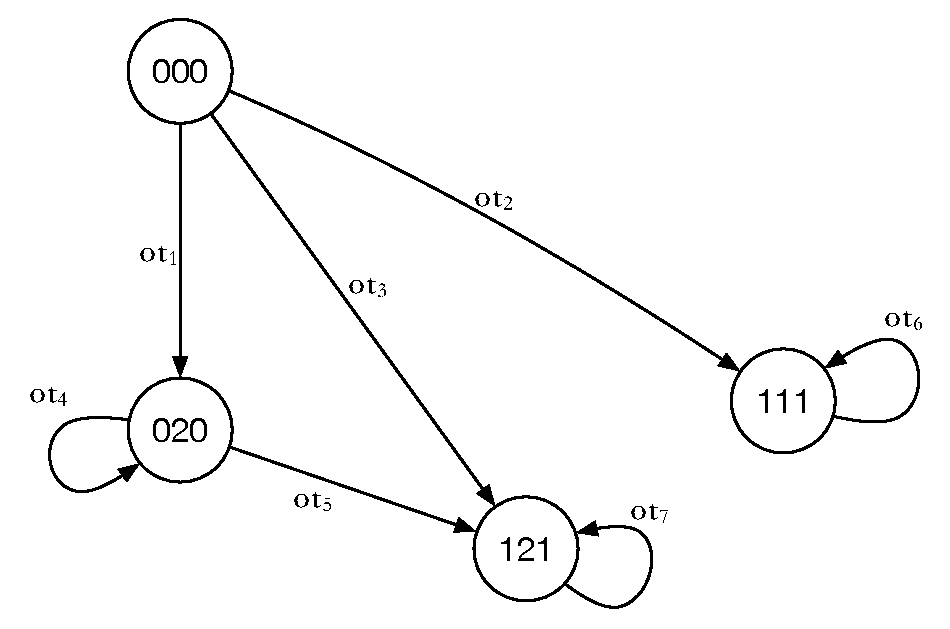
\includegraphics[width=5cm]{XFIG/LOTOSresult}}
  \TODO{Detaisl of some OTs of the FailureTimer}
  
$\begin{array}{@{}r@{}l@{}}
    ot_1  = &\openrule{\{0 \xrightarrow{l}_{C_1} 0\}, ~~\{\xrightarrow{hb_{1}}_P\}, ~~[s_0=0 \!\land\! hb_{1} \neq \delta(x) \!\land\! v_1=hb_{1}]}
    {\ostate{00} \xrightarrow{v_1} \ostate{00}}\\
  \end{array}$

$\begin{array}{@{}r@{}l@{}}
    ot_2  = &\openrule{\{0 \xrightarrow{\delta}_{C_1} 0, 0 \xrightarrow{acc(x)}_{C_2} 1\}, ~~\{\xrightarrow{hb_{2}}_P\}, ~~[s_0=0 \!\land\! hb_{2}=\delta(x) \!\land\! v_2=\underline{\delta(x)}], ~~\{s_0 \xleftarrow{} 1\}}
    {\ostate{00} \xrightarrow{v_2} \ostate{01}}\\
  \end{array}$
  

\caption{The open automaton of the LOTOS formula}  \label{schema:lotos-result}
\end{figure}

%\subsubsection{Result of CCS example}
%\QIN{
%also can present all the possible behavior of that CCS formula with 16 open
%transitions in Fig. ~\ref{schema:ccs-result}, here we omitted the details of open transitions. 
%In this example, there are 32 more transitions detected unsatisfiable by Z3.
%}
%
%\QIN{
%Here we only show one of the result transitions. It presents the value-passing between $a.P$ and $b.Q$ and they are synchronized then
%give out an silent action $\tau$, process $P$ and $Q$ should not work in this case.
%}
%
%\begin{figure}[h]
%  \centerline{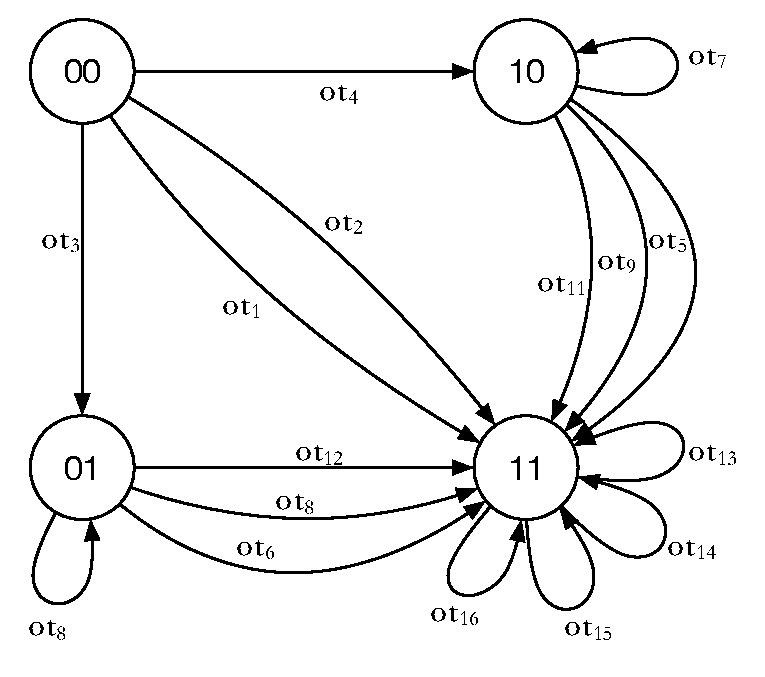
\includegraphics[width=5cm]{XFIG/CCSresult}}
%  
%  $\begin{array}{@{}r@{}l@{}}
%    ot_1  = &\openrule{\{0 \xrightarrow{a}_{C_1} 1, 0 \xrightarrow{b}_{C_2} 1\}, ~~a=!ch_{11}(v_{11}) \!\land\! b=?ch_{11}(v_{11}) \!\land\! a\neq l \!\land\! b\neq r\!\land\! v_1=\tau}
%    {\ostate{00} \xrightarrow{v_1} \ostate{11}}\\
%  \end{array}$
%  
%\caption{The open automaton of the CCS parallel formula}  \label{schema:ccs-result}
%\end{figure}

%% \QIN{
%% To sum up, from the pNets encoding the formulas of given algebra, which inputed by the user, we can exactly construct
%% the open automaton for them. 
%% }


\section{Conclusion and Discussion}
\label{section:conclusion}

In this paper we presented the algorithm for generating an open
automaton representing the semantics of an open pNet, and we described
the implementation of the
algorithm. Our implementation includes two main parts. First, we
compute all the possible open transitions. The actions in pLTS and
hole behaviors are composed in the algorithm while the generation of
predicate need to match the combinations of the subnets with the
synchronization vectors. Some of the open transitions obtained at this
intermediate step, constructed in a structural manner from all
possible combinations of possible logical predicates, may
contain predicates which do not represent any possible concrete
instantiations. 
To get rid of these useless transitions, we use the SMT solver Z3 for checking the
satisfiability of the predicate in each open transition. In
order to do that, we encode into Z3 the action algebra presentation,
the a representation of the predicates, before submitting them to the
Z3 solver. We implemented our algorithm in the VerCors platform and use some
running examples, encoding expressions from various process algebras, to test the
algorithm. Our use-cases show that our encoding
identifies successfully all unsatisfiable open transitions and that
the resulting automaton reflects correctly the expected 
movements of the encoded process expressions.   

Among the questions arising during this work, an important one is the
efficiency of Z3 for our needs. Z3 is famous for being very fast for
solving very large sets of assertions, and this could be important for
us. But we encountered  some problems during the implementation the
checking method using Z3. For example, if the $functions$ and the
$datatypes$ part of the algebra presentation we submit to the solver
are independent with each other, then checking the $assertions$ is a
simple work. However, $functions$ on recursive $datatypes$ make it
more complex, some special rules might be defined by user for the
induction. Also, we need more evidence that dealing with more complex
action algebras, that would involve axiomatizing their data structures
into Z3 theories, will indeed allow us to decide validity of
predicates.
We may also try other automatic theorem provers, depending on the structure of the proofs we need.

\TODO{Change perspective: we are working on the formal extensino of
  BIB architectures, and their semantics in terms of pNets. Then
  bisimulation and model-checking principles adapted to open pNet
  systems are under development}

Naturally, our next goals after the generation of the open automata
will be to model-check, and to check equivalence of  pNets. While
model-checking open automata (with a suitable logic including
predicates on data) seems easy to define, equivalence checking is more challenging.
In previous paper, we
have already found the FH-bisimulation, inspired by~\cite{deSimone85} as a
suitable definition. But usual approaches of bisimulation by partition
refinement does not work easily with symbolic transitions. In a first
step we may want instead to define and implement an algorithm for
checking that a given equivalence relation between open automata 
states is indeed a FH-Bisimulation. Finding automatically a
bisimulation relation or the most general bisimulation will be more
challenging. It appears also that when comparing different pNets with
different structure, strong bisimulation will be too strong a notion,
and that we will have to define proper notions of weak equivalence or
refinements. 

Before that work, we need to reconsider the result open transitions
from our algorithm. The ideal
result that we showed in the bottom part of
Fig.~\ref{schema:lotos-result} is not the one generated by the algorithm,
because the original one contains many intermediate
variables, such as fresh local variables of synchronization
vectors, and fresh result variables of intermediate open transitions.
Such intermediate variables come from the way predicates are
generated, and depends on the particular structure of the pNet. But
they are not significant in the resulting behavior, and should be
eliminated before comparing such behavior with another pNet.
To eliminate the intermediate variables in the predicate, we want to define
the set of the significant variables that we won't eliminate: the
local variables of pLTS transitions, the hole behaviors and the result
action at the top level.
The result of the elimination will be simpler predicates, that can be
successfully compared (e.g. by Z3) within the bisimulation checking
algorithm.



\bibliographystyle{lncs/splncs}

% \bibliography{oasis,biblio}
\bibliography{biblio}

% \newpage
\appendix

\section{More details on the generation algorithm}
\subsection{Algebra specification}
\subsection{Term algebra: type system and static semantics}
Our models rely on a notion of parameterized actions, that are
symbolic expressions using data types and variables. As our model aims
at encoding the low-level behavior of possibly very different
programming languages, we do not want to impose one specific algebra
for denoting actions, nor any specific communication mechanism. So we
leave unspecified the constructors of the algebra that will allow building
expressions and actions. Moreover, we use a generic {\em action interaction}
mechanism, based on unification between two or more action
expressions. This will be used in the semantics of synchronization
vectors to express various kinds of communication or synchronization mechanisms.

\def\Talg{\mathcal{T}_{\Sigma,\P}}
Formally, we assume the existence of a term algebra $\Talg$,
where $\Sigma$ is the signature of the data and action constructors,
and $\P$ a set of variables. Within $\Talg$, we distinguish a set of
data expressions $\mathcal{E}_\P$, including a set of boolean
expressions $\mathcal{B}_{\P}$ ($\mathcal{B}_{\P}\subseteq\mathcal{E}_\P$).
On top of $\mathcal{E}_\P$ we build the action algebra
$\mathcal{A}_\P$, with $\mathcal{A}_P\subseteq\mathcal{T}_\P,
\mathcal{E}_P\cap\mathcal{A}_P=\emptyset$;
naturally action terms will use data expressions as sub-terms.
The function $\vars(t)$ identifies the set of variables in a term
$t\in\AlgT$.


pNets can encode naturally the notion of input actions as found e.g. in value-passing CCS
\cite{Milner89} or of usual point-to-point message passing calculi, but it also allows
for more general mechanisms, like gate negotiation in Lotos, or broadcast
communications.

\subsection{Fresh variables}

%The variables in each synchronization vector are considered local, so
%does the variables of an open transition such as its hole behaviors
%and its result action. So we want rename the variables to make them
%unique on every occurrence of a vector. Similarly, the name given to
%the hole behaviors for each hole or the result action for each open
%transition must be distinct. At the same time, we also hope them still
%readable. Here we rename the variables with a regular format using the fresh function. 

Application of the semantic rules require generating a lot of fresh
names, for different kind of variables. We could use a global name
generator to guarantee unicity, but 
at the same time, we also hope them still
readable. Here we rename the variables with a regular format using the fresh function.
More precisely, the fresh function generates a new name adding a
suffix after the original name. The suffix contains three parts
combined by a colon.  


\begin{definition}[Fresh variable]\label{fresh-variable}
The format of \emph{fresh variable} (renaming) is defined as:
``$\emph{prefix : tree\ index\ :\ counter}$''.
\begin{itemize}
   \item[$\bullet$] $prefix$ identifies the kind of the
     variable. current kinds are: sva (SV action), ra (result action), hb (hole behavior).
   \item[$\bullet$] $tree\ index$ is the index of the node containing the variable in the tree-like structure of the pNet.
   \item[$\bullet$] $counter$ is the current value of the corresponding counter.
\end{itemize}
\end{definition}

%\TODO{Option: Add the process and the vector ids ?}

%$Prefix$ avoids the confusion between variables from different structures with the same name by attaching the type of the structure. $Tree\ index$ is given to every node of the pNets to mention which node the variable belongs to as pNets has a tree-like structure. To each node, the tree index is always a number sequence of the tree index of its higher level and the index of the node in this level at the last. $A\ set\ of\ counters$ is used to count the current times the SV, Hole, subnet invoked, or the number of possible OT generated to provide an identity. 

For example, in the running example, the first possible behavior of
the hole, it doesn't have a name, only have the prefix ``hb''. The
hole is the second subnets of the root node so its ``tree index'' is
``12''. The fresh variable name is ``$\OTvar{:hb:12:1}$''. 
\subsection{Variable managment}
The variables in each synchronisation vector are considered local: for a given pNet expression, we must have fresh local variables for each occurrence of a vector (= each time we instantiate rule Tr2). Similarly the state variables of each copy of a given pLTS in the system, must be distinct, and those created for each application of Tr2 have to be fresh and all distinct. This will be implemented within the open-automaton generation algorithm, e.g. using name generation using a global counter as a suffix.
\subsection{Filtering the behaviour combinations}
\QIN{There is already able to filter some wrong open transitions during the matching.
We can ensure that the synchronization vector is not matched with the subnets if there is only one side not involved.
Then we can remove the transitions from the result of matching according to the condition $\gamma$ where
$\gamma = \bigcup_{i\in I}(v_i\in\eta\land a'_i\in\eta)\lor(v_i\in\eta\land a'_i\in\eta) .$
}
\subsection{Translation to SMTlib input language}
In order to submit satisfiability problems to Z3 (for the predicates
in open transitions), we need to generate SMTlib programs, from the
pNet Algebra presentation and predicates.
More precisely, we need to translate to SMTlib:
\begin{itemize}
  \item the presentation of the action algebra
    (sorts and operators) that is defined for a given language (process calculus, or high level programming language),
    \item for a given pNet, the set of local constants (actions or auxiliary data) that are used in the pLTSs,
    \item for each open transition: the declaration of variables, and
      the predicate (including action expressions).
\end{itemize}

During this translation, in order to guarantee that the generated code
will cause no runtime errors during parsing and execution, we need
to ensure that all objects used in the SMTlib code are properly
declared, and that they are correctly typed.

Note that in principle, such an algebra correspond to a given
high-level language (e.g. a process algebra), and that the algebra
presentation will be defined once and for all in the framework of the
pNet semantics of each specific language.

\paragraph{Algebra presentations}
\begin{definition}
  An Algebra Presentation is a pair $\mathcal{P}=<Sorts,Constrs,Ops>$ where:
  \begin{itemize}
  \item $Sorts$ is a set of Sort names
    \footnote{Later we may want to extend this with Sort constructors,
      like Array or Pair, but this is not needed now}
  \item $Constrs$ is a set of constructor operators, with $Con$ the
    constructor name, and arity: $arity(Con)=n \in \mathbb{N}$,
    and with their signature and their associated selectors,
    of the form: '$Con : (sel_1,sort_1), ... , (sel_n,sort_n) -> sort$'.
    For each argument, the pair $(sel_i,sort_i)$ defines an auxiliary
    operator of name $sel_i$ with signature $sel_i : sort -> sort_i$.
    \item $Ops$ is a set of other (auxiliary) operators, with their
      arity and signature, of the form: $Op : sort_1, ...  sort_n ->
      sort$
      \item $Constrs(sortname), Sels(sortname)$, respectively define the set of
        constructors and selectors of sort $sortname$
  \end{itemize}
  All sorts and operator names must be distinct.\\
  Amongst Constructors, those of arity 0 are called constants, and we
  define $Consts(\mathcal{P}) = \{Con \in Constrs. arity(Con)=0\}$.
\end{definition}


We have a minimal, predefined algebra presentation for all pNets, including
three basic sorts $Bool$, $Action$ and $Int$ and their
operators. Table \ref{Table:predefinedSorts} defines these elements.

In addition, and for convenience, we provide one generic construct for
parameterized actions named FUN, which can accept any number of
arguments of any sort. The result type, though, can only be $Action$,
in order to keep the type-checking simple (see next section).

\begin{table}\caption{\label{Table:predefinedSorts}\leftline{Algebra Presentation: predefined Sorts
  and Operators}}
	\begin{tabular}{p{3cm}p{3cm}p{6cm}}
		\hline\specialrule{0em}{1pt}{1pt}
		Sort & Constructors & Other Operators
                \\\specialrule{0em}{1pt}{1pt}
		\hline\specialrule{0em}{3pt}{3pt}
		Bool    			&
                $\texttt{true},\ \texttt{false}$&
                $\land,\ \lor$
                \\\specialrule{0em}{1pt}{1pt} 
		Action 			&  $\texttt{FUN}$ &
                \\\specialrule{0em}{1pt}{1pt}
		Int 				&
                ${0, \{i, -i\}_{i \in \texttt{Nat}}}$  &
                $- \texttt{(unary)},\ +,\ -
                \texttt{(binary)},\ \times,\ \div, \texttt{etc.}$
                \\\specialrule{0em}{1pt}{1pt}
                \textsl{for any sort} & & $=,\ \ne$
		\\\hline
	\end{tabular}
\end{table}

For a given language, or for a given use-case, the designer can
declare more sorts and operators, using our pNet API.
As an example, a (value-passing) CCS action algebra, where we assume a
single auxiliary value domain ``Data'', can be defined as:

\begin{example}
  \begin{itemize}
    \item[]
    \item $Sorts_{CCS} = \{Action, Channel, Data, Int, Bool\}$
    \item $Constrs_{CCS} =\\
    \texttt{Emit}: 2, \{(Chan\_E:Channel),(Value\_E:Data)\}->Action\\
    \texttt{Receive}: 2, \{(Chan\_R:Channel),(Value\_R:Data)\}->Action\\
    \texttt{Tau}: 0, \{\}-> Action\\
    \texttt{... and all predefined operators}$
  \end{itemize}
\end{example}

Then in pNet API these operators or constants (seemed as non-parameter operators) can be declared as:
\begin{lstlisting}[basicstyle=\footnotesize\ttfamily, language=java, frame=single]
AlgebraSort Action = new AlgebraSortImpl("Action");
AlgebraSort Channel = new AlgebraSortImpl("Channel");
AlgebraSort Data = new AlgebraSortImpl("Data");
Action.addConstructor("Emit", 
	{"Chan_E", "Value_E"}, {Channel, Data});
Action.addConstructor("Receive", 
	{"Chan_E", "Value_E"}, {Channel, Data});
Action.addConstructor("Tau");
\end{lstlisting}

\TODO{[DONE][Xudong]: Give an example of defining $Tau$ and $Emit$ using the (new
  version of) the API}

\paragraph{Expressions}
Once an algebra presentation is defined, we can construct expressions
of the term algebra, using variables and operators:

\begin{definition}
  Let $\mathcal{V}$ be a set of variables. The Term Algebra
  $\Sigma_{\mathcal{P},\mathcal{V}}$ is the set of:
  \begin{itemize}
  \item variables $x \in \mathcal{V}$
  \item terms (or expressions) $op (arg_1, ... , arg_n)$ with $op$ an operator in
  $\mathcal{P}$ of arity $n$, and each $arg_i$ an expression.
  \end{itemize} 
\end{definition}

\paragraph{Constants and variables in pNets and in open transitions}

In addition to the objects defined in the Algebra Presentation, there are
specific objects that are introduced by the pNet construction, and by
the semantic rules used to build the open transitions and their
predicates. This includes, for a pNet $pnet$
\begin{itemize}
\item $Const(pnet)$: Constants from the pLTSs (controllers) transitions: these are
  new constant constructors, usualy of sort Action, local to an
  instance of a controller. The pNet definition requires that all
  these constants are distinct from each other.
\item $SVars(pnet)$: State variables of the controllers. Here also they are required
  to be distinct from those of other controllers.
\item $IVars(pnet)$: Input variables of the controllers.
\item $FVars(pnet,ot)$: Several kinds of ``fresh'' variables, created by application of
  rule Tr2, during the construction of each open transition $ot$:
  Action variables for the behavior of holes and the 
  resulting actions of transitions, variables created during the cloning
  of synchronisation vectors.
\end{itemize}

\def\EPres{\mathcal{P}}
\def\EEnv{\Gamma}

All variable sets above include their sort.
To define the typing rules for expressions and the translation
functions, for any pNet $pnet$ and open transition $ot$, we define an
extended presentation $\EPres_{pnet}$ and environment $\EEnv_{pnet,ot}$ that includes all of the
objects above:

\begin{definition}
  Given an algebra presentation $\mathcal{P}_{pnet}=<Sorts,Constrs,Ops>$ and a pNet $pnet$, we
  construct:
  \begin{itemize}
  \item An extended presentation $\EPres_{pnet}<Sorts,Constrs \cup Const(pnet),Ops>$.
  \item For a given open transition $ot$, an environment
    $\EEnv_{pnet,ot}=SVars(pnet) \cup IVars(pnet) \cup FVars(pnet,ot)$. 
  \end{itemize} 
\end{definition}



\paragraph{Well-formed and well-typed expressions}

The purpose of this section is to define static semantic notions that
will guarantee that the translation to the SMT language will be
correct, i.e. will not yield errors at runtime. This includes
well-formness (all sorts, operators, variables are defined, and
expressions respect the arity of operators), and typing rules. 

\begin{definition}
  Given a presentation $\EPres$ (possibly extended) and an environment $\EEnv$:
  \begin{itemize}
  \item $\EEnv$ is well-formed if all sorts in $\EEnv$ are
    defined in $\EPres$
  \item an expression is well-formed if all its operators are defined
    in $\EPres$, and used with the proper arity, and all its
    variables are defined in $\EEnv$
  \item an expression is well-typed if it can be typed by the typing
    rules in table \ref{table:typing-rules}
  \end{itemize}
\end{definition}

The following judgment, and the typing rules in table
\ref{table:typing-rules} can be used to check both the wellformedness
and well-typing of expressions in a pNet or in an open transition,
given the corresponding $\EPres$ and $\EEnv$.

%\begin{table}\caption{\leftline{Typing judgment for Expressions in Open pNets}}
\vspace{1ex}
\noindent
\begin{tabular}{p{5cm}p{7cm}}
		\hline\specialrule{0em}{3pt}{3pt}
%%		$\EEnv \vdash \diamond$ 					& $\EEnv$ is a well-formed environment 					\\\specialrule{0em}{1pt}{1pt}
%%		$\EEnv \vdash A$ 							& A is a well-formed type in $\EEnv$	 					\\\specialrule{0em}{1pt}{1pt}
		$\EPres,\EEnv \vdash M: A$
                & M is a well-formed term of type A in $\EPres,\EEnv$			\\\specialrule{0em}{1pt}{1pt}
		\specialrule{0em}{3pt}{3pt}\hline
	\end{tabular}
%\end{table}	

\begin{table}\caption{\leftline{Type Rules for Open pNets}}
  \label{table:typing-rules}
	\begin{tabular}{p{5cm}p{5cm}p{2.5cm}}
		\hline\specialrule{0em}{3pt}{3pt}
		%% (Env $\varnothing$) 								
		%% & 										
		%% &					\\\specialrule{0em}{1pt}{1pt}
            %% $\dfrac{ }{\varnothing \vdash \diamond}$			
            %% & %$\dfrac{\EEnv \vdash A ~~ x\ }{\varnothing \vdash \diamond}$
            %% &					\\\specialrule{0em}{3pt}{3pt}
		%% (Type Bool) 										
		%% &(Type Action) 						
		%% &(Type Int)			\\\specialrule{0em}{1pt}{1pt}
		%% $\dfrac{\EPres \vdash Bool~~\EEnv \vdash \diamond}{\EPres,\EEnv \vdash Bool}$ 
		%% & $\dfrac{\EPres \vdash Action~~\EEnv \vdash \diamond}{\EPres,\EEnv \vdash Action}$ 
		%% & $\dfrac{\EPres \vdash Int~~\EEnv \vdash \diamond}{\EPres,\EEnv \vdash Int}$        \\\specialrule{0em}{3pt}{3pt}
		(Var x) 										
		& 						
		&			\\\specialrule{0em}{1pt}{1pt}
		$\dfrac{\EEnv \vdash x:A}{\EPres,\EEnv \vdash x:A}$ 
		&  
		&       		\\\specialrule{0em}{5pt}{5pt}
		\multispan{2} (Binary operators, e.g.: $\land, \lor$ for booleans, $+, -, \times, \div, \le, \ge$ for integers, etc.)								
							
		& 			\\\specialrule{0em}{3pt}{3pt}
		$\dfrac{\EPres \vdash BinOp :: ty1, ty1 \rightarrow ty2 ~~\EEnv \vdash x_1:ty1 ~~\EEnv \vdash x_2:ty1}{\EPres,\EEnv \vdash x_1 ~BinOp~ x_2:ty2}$ 
		& 
		&       		\\\specialrule{0em}{3pt}{3pt}
		\multicolumn{2}{l}{(Unary operators, e.g. $\lnot$ for booleans, - for integers)}	
                
		& 			\\\specialrule{0em}{3pt}{3pt}
		$\dfrac{\EPres \vdash UnOp :: ty1 \rightarrow ty2 ~~\EEnv \vdash x:ty1}{\EPres,\EEnv \vdash Unop~x:ty2}$   
		&&       		\\\specialrule{0em}{5pt}{5pt}
		(Polymorphic EQ and NEQ)							
		&					
		&
                                         \\\specialrule{0em}{3pt}{3pt}
		$\dfrac{\EPres \vdash A  ~~\EEnv \vdash x_1:A ~~\EEnv \vdash x_2:A}{\EPres,\EEnv \vdash x_1 = x_2:Bool}$ 
		& 
		$\dfrac{\EPres \vdash A  ~~\EEnv \vdash x_1:A ~~\EEnv \vdash x_2:A}{\EPres,\EEnv \vdash x_1 \ne x_2:Bool}$ 
		
		&       		\\\specialrule{0em}{5pt}{5pt}
		(Overloaded FUN)							
		&					
		& 			\\\specialrule{0em}{3pt}{3pt}
		$\dfrac{\EPres \vdash \texttt{FUN} :: A_1,...,A_n \rightarrow Action ~~\EPres \vdash A_1~~...~~\EPres \vdash A_n ~~\EEnv \vdash x_1:A_1~~...~~\EEnv \vdash x_n:A_n}{\EPres,\EEnv \vdash \texttt{FUN}(x_1,...,x_n):Action}$ 
		& 
		&			\\
		\specialrule{0em}{5pt}{5pt}\hline
	\end{tabular}
\end{table}	

\begin{remark}
  These rules provide a simple type-checking algorithm: if all
  variables in an expression are known in $\EEnv$, then a bottom-up
  application of the rules will decide whether the expression is
  well-typed, and compute the type of each sub-expression.
\end{remark}

\subsubsection{Map to SMT-LIB language}
The pNet elements, as defined above, can be full translated into
SMT-LIB language, but there are a number of differences in the
structure of the models/langages, so the translation is not trivial.

In this section we shall define separately the translation of the
(extended) algebra presentation for one pNet (so it will be fixed for
the study of one use-case); and the translation of each predicate in
the context of an open-transition of this pNet.

\def\translate{~\lhook\joinrel\longrightarrow}

\vspace{1ex}\noindent
%\begin{table}\caption{\leftline{Mapping}}
	\begin{tabular}{p{3cm}p{9cm}}
		\hline\specialrule{0em}{1pt}{1pt}			
		(Presentation)							
		&								\\\specialrule{0em}{1pt}{1pt}		
		&$Sorts \& Constructors \translate$	declare-datatypes				\\\specialrule{0em}{1pt}{1pt}
		&$Operators \lhook\joinrel\longrightarrow$	declare-function		\\\specialrule{0em}{1pt}{1pt}
		(Predicate)							
		&								\\\specialrule{0em}{1pt}{1pt}
		&$\EEnv ~~\lhook\joinrel\longrightarrow$	declare-const		\\\specialrule{0em}{1pt}{1pt}
		&$Pred ~~\lhook\joinrel\longrightarrow$	 assert		\\\specialrule{0em}{1pt}{1pt}
		&$\texttt{FUN}(x_1,...,x_n)$		\\\specialrule{0em}{1pt}{1pt}
		&$\texttt{pNet expression} ~~\lhook\joinrel\longrightarrow$ SMTLib expression	\\\specialrule{0em}{1pt}{1pt}
		&$...$	\\\specialrule{0em}{1pt}{1pt}
		\specialrule{0em}{1pt}{1pt}\hline
	\end{tabular}
%\end{table}

\smallskip
\ERIC{My plan here is to provide the translation principles as some
  high-level pseudo code, together with precise definition of the
  translation functions of a presentation+environment, and of a
  predicate (including expressions)}

In the following definitions, we use abstract functions corresponding to
SMTlib/Z3 constructs. In practice they can be implemented either as
SMTLib scripting programs, or as calls to the Z3 java API.

\subsubsection{Presentation Translation}
We define here the translation of the algebra presentation, extended
with the constant operators collected from the pNet. It produces the
declaration of sorts (excepted Bool and Int) with their constructors
and selectors as \texttt{declare-datatypes}, and the declaration of
other operators as \texttt{declare-function} constructs.
For sorts, we must distinguish the case of mutually defined sorts
(e.g. edges and vertices in a graph), that must be declared within a
single \texttt{declare-datatypes} construct. For this we define:

\begin{definition}
Define the (strict) order "is-using" between sorts $S1 is-using S2$ iff $S2$
occurs as the sort of one argument in the constructors of $S1$.
\end{definition}

\TODO{[Xudong: this is certainly obsolete?] At the same time, we have
  several internal lists (actually hash 
  maps) \texttt{exprs}, \texttt{funcDecls}, \texttt{sortDatatypes} to
  store the generated Z3 objects with their names for later proofs.} 

\begin{lstlisting}
Let Pres = <Sorts, Constrs, Ops> an extended presentation
(i.e. including the constants from the pnet),
- define MySorts = Sorts \ {Bool, Int}
- compute the strongly connected components in the graph
  of MySorts with respect to the relation is-using
- for each SCC in this graph, construct: 
  dataype-declaration = TrPresentation (Pres, SCC)
- for each other operator op in Ops, construct:
  function-declaration = TrPresentation (Pres, op)
\end{lstlisting}

%\begin{table}\caption{\leftline{Rules for TrPresentation}}
%  \label{table:TrPresentation}
\noindent
\begin{tabular}{p{5cm}p{5cm}p{2.5cm}}
		\hline\specialrule{0em}{3pt}{3pt}
		\multicolumn{2}{l}{One datatype declaration for each SCC}
                
		& 			\\\specialrule{0em}{1pt}{1pt}
		$\dfrac{name=name(Sort) \qquad constrs=Constrs(name) %\qquad sels=Sels(name)
                  \translate constrs}
                       {SCC \translate
                  \texttt{(declare-datatypes () $name$ (map $\translate constrs$))}}$ 

		&&       		\\\specialrule{0em}{1pt}{1pt}
		\multicolumn{2}{l}{Constants: }	
                
		& 			\\\specialrule{0em}{1pt}{1pt}
		$\dfrac{arity(constr)=0}
                       {constr \translate \texttt{name($constr$)}}$
                
		&&       		\\\specialrule{0em}{1pt}{1pt}
		\multicolumn{2}{l}{Other constructors: }	
                
		& 			\\\specialrule{0em}{1pt}{1pt}
		$\dfrac{n = arity(constr) \neq 0 \qquad |sels|=n
                  \qquad sels =  BuildSels(constr)}
                       {constr \translate \texttt{(name($constr$) . sels)}}$
                       
		&&       		\\\specialrule{0em}{1pt}{1pt}
		\multicolumn{2}{l}{Other operators: }	
                
		& 			\\\specialrule{0em}{1pt}{1pt}
		$\dfrac{op : sort_1, ..., sort_n : sort}
                       {op \translate \texttt{(declare-fun name($op$) ($sortname_1
                           ... sortname_n$) $sortname$)}}$
                       
		&&       		\\\specialrule{0em}{1pt}{1pt}
		\multicolumn{2}{l}{Special case of FUN: }	
                
		& 			\\\specialrule{0em}{1pt}{1pt}
		$\dfrac{}
                       {FUN \translate \texttt{map $\translate CollectFunTypes(pNet)$ }}$
                       
		&&       		\\\specialrule{0em}{1pt}{1pt}
		$\dfrac{}
                       {argstypes \translate \texttt{(declare-fun
                           $BuildFunInstance(argstypes)$ (map name
                           $argstypes$) Action) }}$
                       
		&&       		\\\specialrule{0em}{1pt}{1pt}
		\hline
\end{tabular}
%\end{table}

\smallskip
Where:
\begin{itemize}
  \item the $BuildSels$ function, for a constructor with $n$ arguments,
argument sorts $sort_i$, and selector names $sel_i$, builds the list
$\{(sel_i, sort_i)\}_{i\in[1..n]}$.
\item the $CollectFunTypes$ function collects all possible instances
  of the overloaded FUN argument types found in the pNet, as computed by the typing
  rules; and $BuildFunInstance$ use these argument types as suffixes
  to disembiguate 
\end{itemize}


\begin{example}
  For the CCS presentation above, we would get (in SMTLib syntax):
\begin{lstlisting}
  (declare-datatypes Data ())
  (declare-datatypes Channel ())
  (declare-datatypes ()
      ((Action (Emit (Chan\_E Channel) (Value\_E Data))
               (Receive (Chan\_R Channel) (Value\_R Data))
               Tau )))
  \end{lstlisting}
\end{example}

\TODO{Need to add an exemple with 2 instances of FUN}

 
\subsubsection{Predicate translation}

\QIN{Each time we submit each open transition to Z3 module, we translate
  its predicate into Z3 language format and send it for satisfiability
  checking. Every term of the predicate is declared as an
  \texttt{assert} in Z3. A constant action or a parameterized
  expression is easy to get from the internal list storing the objects
  while all the variables are not declared at the beginning. So we
  declare them before the submission of a predicate term with the API
  method conducting \texttt{declare-const}.}

The second part of the translation function is called for each open
transition. More precisely we need here:

\begin{lstlisting}
Let Pres = <Sorts, Constrs, Ops> be the extended presentation
and OT = <Leaves, Holes, Pred, Assign> an open transition.
- compute the environment $\EEnv=\EEnv_{pnet,OT}$ collecting
all variables used in OT
- check that all pLTS labels (action, guard, assignement) in
the transition, the OT predicate, and the OT assignments are
well-formed and well-typed
- for each variable $v$ in $\EEnv$, construct:
  define-const = TrPredicate ($\EEnv,v$)
- turn the predicate into conjunctive normal form
- for each conjunct $P_i$ in the predicate, construct:
  assert = TrPredicate $(P_i)$
\end{lstlisting}

\noindent
\begin{tabular}{p{5cm}p{5cm}p{2.5cm}}
		\hline\specialrule{0em}{3pt}{3pt}
		\multicolumn{2}{l}{Variables}
                
		& 			\\\specialrule{0em}{1pt}{1pt}
		$\dfrac{\EEnv \vdash x:A }
                       {x \translate \texttt{(declare-const x A)}}$
                  
		&&       		\\\specialrule{0em}{1pt}{1pt}
		\multicolumn{2}{l}{Predicate conjunct: }	
                
		& 			\\\specialrule{0em}{1pt}{1pt}
		$\dfrac{}
                       {P_i \translate \texttt{(assert ... }}$
                
		&&       		\\\specialrule{0em}{1pt}{1pt}
		\multicolumn{3}{p{12cm}}{To be completed with translation of
                expressions, including special cases for EQ, NOT\_EQ,
                and FUN }	
                
		 			\\\specialrule{0em}{1pt}{1pt}
		\hline
\end{tabular}
\subsection{Elimination of intermediate variables}
\QIN{
We apply several structural rules to generate the predicates restricting the composition of the subnets by synchronization vectors.
The predicates may contain some redundancy if there are variables in middle level are matching other variables both in lower and higher level at the same time. 
}

We already have the operational semantics of open pNets restricting the open transitions using two rules.
The generated equations in the $predicates$ contain either intermediate variables or ground ones, but what we want is the equation between ground terms. 

\QIN{
We want to reason about the equations to eliminate the redundancy. 
Considering pNet has a special tree-structure, the replacement between equations should be one-way, the direction is from leaves to the top level, until the root pNet node. 
And it is easy to figure out the intermediate variables by the constraint rules.
While it is not needed figure out if an equation is "true" , it can be left to Z3.
}

\begin{definition}[Intermediate Variable]
\paragraph{}
When applying Tr1, we do not collect intermediate variables. Though the result action might be the intermediate one between two result action from the SV if it is not the root of the pNet, it will be determined at the higher level instead of at the leaves.

\begin{description}
	\item[{\bf Using the parameters from Tr1:}]
\end{description}

\[ InterVar(OT) = \emptyset \]

\paragraph{}
When it comes to a pNet node, all the variables from the sources mentioned above should be contained in the $InterVar$ together with the intermediate variables from the subnets. Whatever its subnet is a pLTS or pNets. At the same time, the subnet's result action should be add into the $InterVar$.

If the result of the SV also occurs in its parameters, it means the action from the subnet will be propagated as the result action of the open transition on this level through this SV result action. So it is also the intermediate variable in such situation.

\begin{description}
	\item[{\bf Using the parameters from Tr2:}]
\end{description}
\[ InterVar(OT) = \bigcup_{m\in I_k}{InterVar(OT_m)}  \bigcup_{m\in I_k}{\{v_m\}} \cup{InterVar(SV_k)} \]
$$ InterVar(SV_k)=\left\{
\begin{aligned}
\emptyset & , & \alpha_{k}^{'} \not\in \bigcup_{m\in I_k \uplus J_k}{\{\alpha_{m}\}}\\
{\alpha_{k}^{'}} & , & \alpha_{k}^{'} \in \bigcup_{m\in I_k \uplus J_k}{\{\alpha_{m}\}}
\end{aligned}
\right.
$$

\begin{itemize}
	\item $OT$ is an open transition.
	\item $I, J$ is the set of indices.
	\item $k$ is the indices of the synchronization vectors.
	\item $SV$ is the set of the synchronization vectors.
	\item $Vars()$ is the function that gets all the variables in the object.
	\item $\alpha$ and $\alpha^{'}$ is the element of the  the synchronization vector.
\end{itemize}
\end{definition}

Definition of the intermediate variable shows that elimination should be done every time Tr2 is applied.

%\texttt{\\
%1. Classify the ground and intermediate variables.
%\begin{itemize}
%    \item (1) The predicates of the subnets: The result actions of the sub-OTs. Others are ground.
%    \item (2) The chosen synchronization vector: If the result is also one of the elements, it is also the intermediate variable. Otherwise, all of the parameters are ground.
%    \item (3) Hole behaviors: Ground.
%    \item (4) The result action: Not sure. But it must be ground if it is on the root node.
%\end{itemize}
%2. Using a list {\em equations} to store the equations containing the intermediate variable. {\em equations} is a hasp map storing the corresponding ground terms of the variable by its name. Its structure likes <String, List<Expression> >. It will be updated during the later deduction .\\
%3. The guards from the subnets are kept, waiting for further substitution.\\
%4. Deduct out the new equations using the redundant Pred got in matching().\\
%    Checking two sides of the equations.
%\begin{itemize}
%   \item If both are ground, then generate a new equation with them, add it to Pred.
%   \item If the right-hand-side or left-hand-side is intermediate, then find the ground term of it from the list then generate a new equation and add it to Pred.
%   \item If both are intermediate, then check the list {\em equations}
%   	\begin{itemize}
%  		\item If list contain both lhs and rhs, then get the corresponding ground terms of them, generate the new equation with the ground terms. Add it to Pred.
%   		\item If list only contain lhs, store the rhs in {\em equations} with lhs's corresponding ground terms.
%   		\item If list only contain rhs, store the lhs in {\em equations} with rhs's corresponding ground terms.
%   		\item Otherwise, skip this turn.
%         \end{itemize}
%\end{itemize}
%5. Search the inter in the guards if it is found, subsititute it with the ground. Then conduct step 2 again.\\
%}

\paragraph{Term Rewriting Rules}
Predicates already have a format declaring what it verifies. According to that previous work, we define the predicates.
Let $\mylangle\overline{\pNet},\overline{S},\symb{SV}_k^{k\in K} \myrangle$
be a pNet. Choose a synchronisation vector $SV=clone(SV_k) ={(a'_i)}^{i\in I}, {(b'_j)}^{j\in J}\rightarrow v' \, ,G_k $, for $k\in K$. The
predicate $\Pred$ relating
the actions of the involved sub-pNets and the resulting actions.
\begin{definition}[Predicate]
\[\Pred(SV, \overline{\pNet},\overline{S}, v) = 
\begin{array}{l}
\forall {(a'_i)}^{i\in I},
{(b'_j)}^{j\in J},v'.
\\
v_m=a'_i\land \, b_j=b'_j \land v=v' \land G_k
\end{array}\]
\end{definition}
\QIN{
The new predicates introduce more hypotheses for term rewriting. However, not every variable can be substituted. 
Here we introduce several rewriting rules.
}

\begin{align*}
   &v_m=a'_i \land v_m=v'_m \rightarrow a'_i = v'_m &[RL-1]\\\\
   &v_m=a'_i \land v=v' \rightarrow v_m=v ~~ \texttt{if} ~~ a'_i = v', ~~ a'_i,v' \in InterVar &[RL-2]\\\\
   &v_m=foo'_i(a_1,...,a_p,...,a_n) \land v=v' \rightarrow v_m=foo'_i(a_1,...,v,...,a_n) \\ 
   &\hspace{15em}\texttt{if} ~~ a_p = v', ~~ a_p,v \in InterVar &[RL-3]\\\\
   &b_j=b'_j \land v=v' \rightarrow b_j=v ~~ \texttt{if} ~~ b'_j = v', ~~ b'_j,v' \in InterVar &[RL-4]\\\\
   &b_j=foo'_i(a_1,...,a_p,...,a_n) \land v=v' \rightarrow b_j=foo'_i(a_1,...,v,...,a_n) \\ 
   &\hspace{15em}\texttt{if} ~~ a_p = v', ~~ a_p,v \in InterVar &[RL-5]\\\\
\end{align*}

\QIN{
Rule RL-1 applies on when the result action of subnets matching other arguments of the chosen SV. It merges the predicates from the subnets with the new generated predicates.
Rule RL-2 shows that if the result of the SV is also in its arguments, we can straightly get an equation between the subnet action and  the result action. RL-3 is the situation that there is an expression instead of a variable contains an intermediate argument. The substitution will only occur on the argument.
Actually, what happened is similar if there is a hole behavior instead of a subnet result action attending in the equation. So we get RL-4 and RL-5. However, every hole behavior should be kept through out the computing. That's why there no rule similar to the RL-1 for hole behaviors.
}
\section{Full examples}
\TODO{May be we use two architecture examples here, a simpler one,
  before the Failure Timer ?}
\subsection{A very simple architecture}
\subsection{Full input for the FailureTimer architecture}
\subsection{Full output for the FailureTimer open automaton}
\subsection{Scaling up: several subsystems on the same bus}

\end{document}
